\documentclass[12pt,a4paper]{report}

\usepackage[utf8]{inputenc}
\usepackage{graphicx}
\usepackage{hyperref}
\usepackage{amsmath}
\usepackage{booktabs}
\usepackage{geometry}
\usepackage{hyperref}
\usepackage{setspace}
\usepackage{titlesec}
\usepackage{titling}
\usepackage{listings}
\usepackage{xcolor}
\usepackage{natbib}
%\usepackage[toc]{glossaries}
\usepackage[acronym]{glossaries}
\usepackage{pgfplots}
\usepackage{pgfplotstable}



\usepackage{fancyhdr}
\pagestyle{fancy}
\fancyhf{}
\fancyhead[R]{\makebox[\textwidth][r]{Enhancing Fraud Detection in Bank Accounts}}
\fancyfoot[C]{\thepage}
\renewcommand{\headrulewidth}{0pt}



\lstdefinestyle{mystyle}{
    backgroundcolor=\color{lightgray!20},   % Choose a light background color
    basicstyle=\ttfamily\small,             % Set the font and size
    keywordstyle=\color{blue},              % Color keywords in blue
    stringstyle=\color{red},                % Color strings in red
    commentstyle=\color{green!60!black},    % Color comments in green
    numberstyle=\tiny\color{gray},          % Line numbers style
    numbers=left,                           % Position of line numbers
    numbersep=5pt,                          % Distance of line numbers from the code
    frame=single,                           % Add a frame around the code
    breaklines=true,                        % Line breaking
    captionpos=b,                           % Caption position
    language=Python                         % Language for syntax highlighting
}
\lstset{style=mystyle}

\geometry{a4paper, top=2cm, bottom=2cm, left=2cm, right=2cm}
\setstretch{1.5}

% Chapter, section, and subsection formatting
\titleformat{\chapter}[block]{\normalfont\huge\bfseries}{\thechapter}{1em}{}
\titleformat{\section}[block]{\normalfont\Large\bfseries}{\thesection}{1em}{}
\titleformat{\subsection}[block]{\normalfont\large\bfseries}{\thesubsection}{1em}{}
\titlespacing*{\chapter}{0pt}{0pt}{12pt}
\titlespacing*{\section}{0pt}{12pt}{6pt}
\titlespacing*{\subsection}{0pt}{12pt}{6pt}

% Footnotes font size
\makeatletter
\renewcommand\footnoterule{%
    \kern-3\p@
    \hrule\@width\columnwidth
    \kern2.6\p@}
\renewcommand\@makefntext[1]{%
    \noindent\makebox[1.8em][r]{\@makefnmark}#1}
\renewcommand{\footnotesize}{\fontsize{10pt}{12pt}\selectfont}
\makeatother

% title page
\renewcommand{\maketitle}{
    \begin{titlepage}
       \noindent
        \vspace*{1cm}
        \begin{center}
            % Centered logo
            \includegraphics[width=0.5\textwidth]{iu_Logo_EN_black_RGB_horizontal.jpg}\\[0.5cm]
    
            \textbf{\fontsize{14pt}{16pt}\selectfont Master Thesis}
            \vspace{1.5cm}
    
            \textbf{\fontsize{14pt}{16pt}\selectfont IU University of Applied Sciences}
            \vspace{0.5cm}
    
            \textbf{\fontsize{14pt}{16pt}\selectfont Study programme: Data Science}
            \vspace{2.0cm}
    
            \textbf{\fontsize{14pt}{16pt}\selectfont Enhancing Fraud Detection in Bank Accounts Through Machine Learning: A Case Study Using the BAF Suite}
            
            \vspace{2.0cm}
            \textbf{\fontsize{14pt}{16pt}\selectfont Volkan Karaarslan}\\
            \vspace{0.5cm}
            \textbf{\fontsize{14pt}{16pt}\selectfont Enrolment number: 92114860}\\
            
            \vspace{0.5cm}
            
            \textbf{\fontsize{14pt}{16pt}\selectfont Bernhard-Letterhaus Str. 25}\\
            \vspace{0.5cm}
            \textbf{\fontsize{14pt}{16pt}\selectfont 41466 Neuss}
            
        \end{center}
        
        % Add lines at the bottom of the title page, beginning from left margin
        \vspace*{\fill}
        \noindent
        \textbf{\fontsize{14pt}{16pt}\selectfont Supervisor: Prof. Robert Graf}\\
        \textbf{\fontsize{14pt}{16pt}\selectfont Date of submission: 1st September 2024}
    \end{titlepage}
}

\makeglossaries
\newacronym{adasyn}{ADASYN}{Adaptive Synthetic Sampling Approach for Imbalanced Learning}
\newacronym{ai}{AI}{Artificial Intelligence}
\newacronym{auc}{AUC}{Area Under the Curve}
\newacronym{baf}{BAF}{Bank Account Fraud}
\newacronym{cart}{CART}{Classification and Regression Trees}
\newacronym{crispdm}{CRISP-DM}{Cross-Industry Standard Process for Data Mining}
\newacronym{ctgan}{CTGAN}{Conditional Tabular Generative Adversarial Network}
\newacronym{dl}{DL}{Deep Learning}
\newacronym{dm}{DM}{Data Mining}
\newacronym{drl}{DRL}{Deep Reinforcement Learning}
\newacronym{eda}{EDA}{Exploratory Data Analysis}
\newacronym{gan}{GAN}{Generative Adversarial Network}
\newacronym{iu}{IU}{Interpretation Unit}
\newacronym{mb}{MB}{Megabyte}
\newacronym{ml}{ML}{Machine Learning}
\newacronym{nc}{NC}{Normalized Cut}
\newacronym{ndcg}{NDCG}{Normalized Discounted Cumulative Gain}
\newacronym{ndcg@k}{NDCG@k}{Normalized Discounted Cumulative Gain at the Position k}
\newacronym{nn}{NN}{Neural Networks}
\newacronym{os}{OS}{Operating System}
\newacronym{rdqn}{RDQN}{Reinforcement Deep Q-Network}
\newacronym{roc}{ROC}{Receiver Operating Characteristic}
\newacronym{rus}{RUS}{Random Under Sampling}
\newacronym{smote}{SMOTE}{Synthetic Minority Over-sampling Technique}
\newacronym{smotenc}{SMOTE-NC}{Synthetic Minority Over-sampling Technique for Nominal and Continuous}
\newacronym{zip}{ZIP}{Zone Improvement Plan}

\begin{document}

\maketitle



\chapter*{} % Empty chapter to avoid numbering and title
\vfill
\begin{center}
    \textbf{\large Acknowledgments}
\end{center}

\vspace{1cm} % Optional: Adjust spacing between the title and the text

I would like to express my deepest gratitude to those who have supported me throughout the completion of this thesis.\\

First and foremost, I am profoundly grateful to my thesis supervisor, Prof. Graf, for his invaluable guidance, insightful feedback, and unwavering support throughout this research. His expertise and dedication have been instrumental in shaping this work, and I am deeply appreciative of the time and effort he has invested in helping me reach this milestone.\\

I would also like to extend my heartfelt thanks to my wife, Sevim, whose love, patience, and encouragement have been a constant source of strength. Her unwavering belief in me and her understanding during the long hours of work have been essential to the completion of this thesis. I am forever grateful for her support and companionship.\\

Thank you both for your invaluable contributions and support on this journey.

\vfill % Pushes the content to the center vertically
\pagenumbering{gobble}
\newpage % Moves to the next page if needed


\begin{abstract}
This thesis explores the application of machine learning techniques in detecting fraudulent activities within bank accounts using the \acrshort{baf} \href{https://www.kaggle.com/datasets/sgpjesus/bank-account-fraud-dataset-neurips-2022/code}{Suite}. It aims to develop and evaluate a machine learning model for fraud detection, thereby improving detection accuracy, increasing working efficiency, and mitigating social inequities caused by biased predictions.
\end{abstract}

\printglossary[type=\acronymtype, title=Abbreviations]
\pagenumbering{gobble}

%\printglossary
\clearpage

\tableofcontents

\pagenumbering{gobble}


\clearpage


\chapter{Introduction}

\pagenumbering{arabic}

\section{Background}
Fraud detection has become increasingly critical in the financial sector due to the significant rise in fraudulent activities. Banks and financial institutions are particularly vulnerable to fraud, which can result in substantial financial losses and damage to reputation. Traditionally, fraud detection systems relied on rule-based methods, which, although effective to some extent, often fail to adapt to new and sophisticated fraudulent techniques.\\


With the advent of machine learning, there has been a paradigm shift in the approach to fraud detection. Machine learning models, with their ability to learn from vast amounts of data and identify patterns, offer a promising solution to detecting fraudulent activities (\citealp[p.4]{bao2020detecting}). The \acrshort{baf} \href{https://www.kaggle.com/datasets/sgpjesus/bank-account-fraud-dataset-neurips-2022/code}{Suite} is a synthetic bank account data set that may be used to test fraud detection capabilities (\citealp{jesus2022turning}). However, the implementation of these models must also consider fairness, ensuring that the models do not perpetuate or exacerbate existing biases, thereby fostering trust and ethical use of technology in financial services (\citealp[p.114]{barocas2023fairness}; \citealp[p.12]{mehrabi2021survey}).\\





\section{Problem Statement and Research Objectives}
Despite the advancements in machine learning, fraud detection in banking remains a challenging task. The primary issues include the imbalance in datasets, with fraudulent transactions being significantly fewer than legitimate ones, and the need for models that are both accurate and interpretable. Moreover, there is a critical need to ensure that these models are fair and do not reinforce existing biases, which can lead to social inequities \citep{corbett2023measure}.\\



The primary objectives of this thesis are:
\begin{enumerate}
    \item To explore the application of machine learning techniques in detecting fraudulent activities within bank accounts using the \acrshort{baf} \href{https://www.kaggle.com/datasets/sgpjesus/bank-account-fraud-dataset-neurips-2022/code}{Suite}.\\
    \item To develop and evaluate a machine learning model for fraud detection using the \acrshort{baf} \href{https://www.kaggle.com/datasets/sgpjesus/bank-account-fraud-dataset-neurips-2022/code}{Suite}, thereby improving detection accuracy, increasing working efficiency, and mitigating social inequities caused by biased predictions.
    \item To investigate the interpretability, reliability, and fairness of the developed model to ensure practical applicability in real-world scenarios.
\end{enumerate}


\section{Significance of the Study}
The significance of this study lies in its potential to enhance the current fraud detection systems used in banking. By leveraging advanced machine learning techniques, this research aims to develop a more accurate, efficient, and fair fraud detection model. This model could significantly reduce financial losses for banks and improve the overall security of financial transactions.\\

Furthermore, the focus on model interpretability and fairness addresses critical ethical considerations in machine learning. By ensuring that the model’s decisions are transparent and unbiased, this research contributes to the broader goal of developing fair and trustworthy \acrshort{ai} systems. The findings from this study could also be applicable to other domains where fraud detection is crucial, such as insurance and e-commerce. Ensuring fairness in machine learning models is essential for fostering trust and promoting ethical practices in technology \citep{barocas2023fairness}; \citep{mehrabi2021survey}.\\

\clearpage

\section{Thesis Structure}
The remainder of this thesis is structured as follows:

\section{Thesis Structure}
The remainder of this thesis is structured as follows:

\begin{itemize}
    \item \textbf{Chapter 2: Literature Review} - In this chapter, we provide an overview of the existing research on machine learning applications in banking, fraud detection, and the challenges associated with model interpretability, reliability, and fairness. We critically examine relevant studies to identify research gaps and establish the rationale for our study.

    \item \textbf{Chapter 3: Methodology} - This chapter outlines the methodology employed in our research, including the \acrshort{crispdm} framework, data preprocessing techniques, and the development and evaluation of machine learning models. We detail the systematic approach taken, from data understanding through to model deployment, to ensure the robustness of our analysis.

    \item \textbf{Chapter 4: Data Description and Analysis} – In this chapter, we describe the dataset used in the study, detailing data collection methods, feature descriptions, and initial data analyses. We also discuss the data preparation steps undertaken, including handling missing values, feature elimination, and encoding of categorical features, which are critical for effective model training.

    \item \textbf{Chapter 5: Exploratory Data Analysis} - Here, we present our exploratory analysis of the dataset, focusing on identifying key patterns and trends. We analyze fraud rates across various categories, such as customer demographics and transaction types, to uncover insights that guide the development of our models.

    \item \textbf{Chapter 6: Feature Selection} - This chapter discusses our approach to feature selection, including correlation analysis and combined feature evaluation techniques. We explain how this process enhances model performance and reduces computational complexity, thereby ensuring that our models are both efficient and effective.

    \item \textbf{Chapter 7: Model Development} – In this chapter, we detail the development of various machine learning models, including Logistic Regression, XGBoost, and Balanced Random Forest. We evaluate these models using performance metrics such as accuracy, precision, recall, and F1-score, highlighting the trade-offs associated with each approach.

    \item \textbf{Chapter 8: Model Fairness Analysis} – We analyze the fairness of the developed models using specific metrics, including Demographic Parity Difference and Equalized Odds Difference. This chapter explores strategies for mitigating biases to ensure that our models do not unfairly impact specific demographic groups.

    \item \textbf{Chapter 9: Enhancing Model Fairness Through Threshold Tuning and Advanced Techniques} - This chapter examines advanced methods for improving model fairness, such as threshold tuning and reweighting. We investigate the impact of these techniques on model performance and fairness, aiming to identify the optimal balance.

    \item \textbf{Chapter 10: Advanced Model Optimization and Performance Enhancement} - In this chapter, we explore advanced optimization techniques, including hyperparameter tuning and the implementation of cutting-edge models such as LightGBM. We assess the impact of these enhancements on the overall performance and reliability of our models.

    \item \textbf{Chapter 11: Results and Discussion} - This chapter presents the findings of our research, synthesizing the performance results of different machine learning models and the effects of various preprocessing, tuning, and fairness techniques. We provide a critical discussion of the results in the context of the study’s objectives.

    \item \textbf{Chapter 12: Conclusion} - In the concluding chapter, we summarize the key findings of our research, discuss the implications for practice, particularly within the banking sector, and propose directions for future research. We highlight the contributions of our study to the field of fraud detection and machine learning.
\end{itemize}





\chapter{Literature Review}
Machine learning has revolutionized various industries, including banking, by providing tools and techniques to analyze large volumes of data and extract meaningful patterns. Its applications in banking encompass credit scoring, customer segmentation, risk management, and fraud detection \citep[p. 3034]{bao2020detecting, pan2024machine, hashemi2022fraud}. The ability of machine learning algorithms to learn from historical data and improve their performance over time makes them ideal for dynamic and complex environments like financial services.

\section{Applications of Machine Learning in Banking}
Machine learning techniques have been extensively applied in fraud detection within the banking sector. Studies such as those by Bao et al. and Seera et al. demonstrate the effectiveness of ensemble learning models and intelligent payment card fraud detection systems, respectively \citep{bao2020detecting, seera2024intelligent}. Further, Pan and Hashemi et al. highlight the importance of feature engineering and hyperparameter tuning in enhancing model performance for fraud detection \citep{pan2024machine, hashemi2022fraud}.\\

Numerous studies have reviewed various techniques for fraud detection. Chaudhary et al. provided an extensive review, combining data mining with machine learning for improved fraud detection accuracy \citep{chaudhary2012review}. Similarly, John et al. emphasized real-time fraud detection through data mining techniques \citep{john2016realtime}. Bakhtiari et al. explored ensemble learning methods, achieving high performance through combining LightGBM and LiteMORT algorithms \citep{bakhtiari2023credit}. Prabowo et al. and Wei et al. discussed the significance of big data analytics and the ContrastMiner algorithm for online banking fraud detection \citep{prabowo2016learning, wei2013effective}.\\

\section{Fraud Detection and Machine Learning}
The increasing attention to machine learning for fraud detection is due to its ability to analyze large datasets and identify patterns indicative of fraudulent behavior. This section reviews studies like those of Jesus et al. and Pombal et al., focusing on the challenges of biased and imbalanced datasets \citep{jesus2022turning, pombal2022understanding}. Additionally, techniques such as SMOTE introduced by Chawla et al. have been pivotal in addressing imbalanced data scenarios in fraud detection \citep{chawla2002smote}.\\

Hashemi et al. presented a comprehensive approach to fraud detection by leveraging Bayesian optimization and weight-tuning hyperparameters to address unbalanced data issues. Their experiments with CatBoost, XGBoost, and LightGBM, as well as a majority voting ensemble method, demonstrated significant improvements in performance metrics such as ROC-AUC, precision, recall, and F1-score \citep[p. 3034]{hashemi2022fraud}.\\

Chaudhary et al. reviewed various techniques used in credit card fraud detection, highlighting the effectiveness of combining data mining techniques with machine learning to improve fraud detection accuracy and reduce false alarm rates. Their review underscores the importance of continuous advancements in fraud detection methodologies to keep up with evolving fraud tactics \citep[p. 39]{chaudhary2012review}.\\

John et al. emphasized real-time fraud detection through data mining techniques, including association, clustering, forecasting, and classification. Their research highlights the significance of analyzing customer data in real-time to identify fraudulent patterns and implement necessary authentication measures to prevent fraud \citep[p. 1186]{john2016realtime}.\\

Bakhtiari et al. explored the use of ensemble data mining methods for credit card fraud detection, demonstrating the effectiveness of combining LightGBM and LiteMORT algorithms. Their study achieved high accuracy and efficiency in detecting fraudulent transactions through the use of ensemble averaging methods \citep[p. 29057]{bakhtiari2023credit}.\\

Prabowo et al. provided a systematic literature review on learning fraud detection from big data in online banking transactions, identifying critical algorithms and emphasizing the importance of big data analytics in enhancing fraud detection capabilities in online banking \citep[p. 127]{prabowo2016learning}.\\
\\

Wei et al. developed an effective online banking fraud detection framework, introducing the ContrastMiner algorithm to efficiently mine contrast patterns. Their research demonstrated higher accuracy and lower alert volume compared to traditional methods, highlighting the effectiveness of their approach in handling extremely imbalanced data \citep[p. 449]{wei2013effective}.\\

El Bouchti et al. showcased the potential of deep reinforcement learning \acrshort{drl} in banking fraud detection. Their study highlighted the efficiency of \acrshort{drl} in learning optimal policies from large datasets, leading to significant improvements in detection accuracy and robustness \citep[p. 58]{el2017fraud}.\\

Vashistha et al. proposed a robust framework for fraud detection in banking using \acrshort{ml} and \acrshort{nn}, utilizing various advanced techniques and achieving 100\% accuracy with Random Forest, XGBoost, LightGBM, and Decision Trees. Their approach effectively balances datasets and improves detection performance, showcasing significant advancements in fraud detection methodologies \citep[p. 201]{vashistha2024robust}.\\

Tekkali and Natarajan developed the \acrshort{rdqn} model, which integrates deep reinforcement learning with rough set theory for digital transactional fraud detection. This model improves both accuracy and processing time by selecting the best features and leveraging an ensemble of deep neural networks and reinforcement learning \citep[p. 5313]{tekkali2023rdqn}.

Gandhar et al. reviewed the latest \acrshort{ml} and \acrshort{dl} techniques for fraud detection, emphasizing the importance of supervised, unsupervised, and reinforcement learning approaches. Their study discussed the strengths and weaknesses of various methods, the challenges of imbalanced datasets, adversarial attacks, and model interpretability, and provided a comprehensive overview of the field \citep[p. 1]{gandhar2024fraud}.\\

\clearpage
\section{Interpretable Machine Learning}
Interpretability of machine learning models is crucial, especially in high-stakes domains like banking. Stakeholders need to understand how and why a model makes certain decisions to trust and effectively utilize its predictions. Interpretable models can help identify biases, ensure compliance with regulations, and provide insights into fraud patterns \citep[p.114]{barocas2023fairness}.\\

Techniques such as decision trees, rule-based systems, and post-hoc interpretability methods are often employed to enhance model transparency. Barocas, Hardt, and Narayanan argue that model interpretability is essential for ensuring transparency and trust in machine learning systems. They discuss various techniques for enhancing interpretability, such as feature importance analysis and model-agnostic methods \citep[p.114]{barocas2023fairness}.\\

Mehrabi et al. surveyed bias and fairness in machine learning, highlighting the need for interpretable models to address ethical and legal considerations in automated decision-making \citep[p.12]{mehrabi2021survey}. They emphasize that interpretable models can help identify and mitigate biases, contributing to fairer and more transparent systems.\\

Molnar provides a comprehensive guide on making black box models explainable, discussing various interpretability techniques such as feature importance, accumulated local effects, and Shapley values. Molnar emphasizes the necessity of model-agnostic methods for interpreting complex models and highlights their strengths and weaknesses in different contexts \citep[p.1]{molnar2020interpretable}.\\

Du et al. categorize techniques for interpretable machine learning into intrinsic and post-hoc interpretability, each with global and local approaches. They highlight the importance of meaningful explanations to avoid artifacts and emphasize the multidisciplinary nature of interpretable machine learning, involving efforts from computer science, human-computer interaction, and social science \citep[p.68]{du2019techniques}.\\

Murdoch et al. define interpretability in the context of machine learning and introduce the predictive, descriptive, relevant framework for discussing interpretations. They categorize interpretation methods into model-based and post-hoc, providing numerous real-world examples to demonstrate the framework's application. Their work emphasizes the importance of human audiences in evaluating interpretability and suggests directions for future research \citep[p. 22071]{murdoch2019definitions}.\\

Gilpin et al. provided an overview of interpretability in machine learning, discussing various explanatory methods and highlighting the need for explanations to ensure fairness, identify potential biases, and validate model performance. Their survey covers foundational concepts of explainability, classifies existing literature, and suggests future research directions for explainable AI \citep[p. 80]{gilpin2018explaining}.

\section{Reliable Machine Learning}
Ensuring the reliability and consistency of machine learning models is vital for their successful deployment in fraud detection. Reliability can be enhanced through robust model validation, continuous monitoring, and regular updates to the model based on new data. It is also important to consider the ethical implications of model decisions and strive for fairness to prevent social inequities \citep[p.12]{mehrabi2021survey}.\\

Fairness-aware machine learning aims to create models that provide equitable outcomes across different demographic groups, thereby promoting ethical AI practices \citep[p.1]{corbett2023measure}. He et al. developed the \acrshort{adasyn} technique for adaptive synthetic sampling, which improves the learning of minority classes in imbalanced datasets. This method enhances model reliability by ensuring that minority classes are adequately represented during training \citep[p.1325]{he2008adasyn}.\\

Xu et al. proposed the use of conditional \acrshort{gan}s for modeling tabular data, which can generate high-quality synthetic datasets for training robust machine learning models. Their approach addresses the challenges of data scarcity and imbalance, contributing to more reliable fraud detection systems \citep[p.42]{xu2019modeling}.\\

Cooper discusses the importance of balancing randomness and arbitrariness in machine learning systems to enhance their reliability at scale. The study highlights key lessons and strategies for ensuring that machine learning models remain robust and trustworthy in diverse and dynamic environments. Emphasizing the need for systematic evaluation and deployment practices, the research provides valuable insights for developing reliable AI systems in high-stakes domains like banking \citep{cooper2024between}.

\section{Fairness in Machine Learning}
Fairness in machine learning (ML) is a critical aspect that aims to ensure that algorithmic decisions do not systematically disadvantage certain groups based on sensitive attributes such as race, gender, or socio-economic status. Achieving fairness in ML involves addressing various forms of biases that can arise from the data collection process, model training, and deployment. Biases in the data, which often reflect historical and societal prejudices, can lead to discriminatory outcomes when these biases are learned and perpetuated by machine learning models. For example, if historical hiring data reflect gender bias against women, a machine learning model trained on such data may continue to disadvantage female applicants, thereby reinforcing existing inequalities \citep{barocas2023fairness}. Therefore, it is essential to incorporate fairness considerations at every stage of the machine learning pipeline to mitigate these biases and ensure equitable outcomes.\\

Moreover, the concept of fairness in ML is multifaceted and can be understood through different theoretical and practical lenses. Several fairness criteria have been proposed in the literature, including demographic parity, equalized odds, and disparate impact. These criteria address various aspects of fairness, such as ensuring that different groups have similar probabilities of being selected by the model, or that errors are evenly distributed across groups \citep{barocas2023fairness}. However, these criteria can sometimes be in conflict, making it challenging to satisfy all fairness requirements simultaneously. Furthermore, fairness interventions, such as reweighting training data or adjusting decision thresholds, must be carefully designed to avoid unintended consequences that could exacerbate existing disparities or create new forms of unfairness. As such, ongoing research and interdisciplinary collaboration are crucial to developing robust and context-sensitive approaches to fairness in machine learning, ensuring that technological advancements contribute positively to social equity \citep{barocas2023fairness}.










\chapter{Methodology}

\section{CRISP-DM Framework}
The \acrshort{crispdm} (Cross-Industry Standard Process for Data Mining) methodology provides a structured approach for data mining and machine learning projects. It includes six phases: Business Understanding, Data Understanding, Data Preparation, Modeling, Evaluation, and Deployment. Each phase is essential for the successful development and implementation of machine learning models.\\

\begin{figure}[h]
    \centering
    \includegraphics[width=0.5\textwidth]{crispdmdiagram.png}
    \caption{CRISP-DM Framework \textit{Source: \cite{jensen_crispdm_image}}}
    \label{fig:crispdm}
\end{figure}

\noindent


\subsection{Business Understanding}
The first phase involves defining the business objectives and requirements for the fraud detection model within the \acrshort{baf} \href{https://www.kaggle.com/datasets/sgpjesus/bank-account-fraud-dataset-neurips-2022/code}{Suite}. The primary goal is to enhance machine learning (ML) research by providing a realistic, large-scale suite of tabular datasets focused on fraud detection in bank account applications \citep{jesus2022turning}. The dataset suite was developed by Feedzai researchers to simulate real-world scenarios, ensuring that the models can handle diverse and challenging conditions. The BAF suite data sheet can be found in this  \href{https://github.com/feedzai/bank-account-fraud/blob/main/documents/datasheet.pdf}{link}.\\



\subsection{Data Understanding}
In this phase, we analyzed the structure and characteristics of the dataset. Given the nature of fraud detection, the dataset is highly imbalanced. The fraudulent transactions are significantly fewer than legitimate ones.  Since ``fraud\_bool'' was the target variable, we performed a classification task to identify fraudulent transactions.\\

We started by importing the data from the CSV file and examining its structure. Next, we conducted exploratory data analysis and created visualizations to better understand the data. A detailed exploratory data analysis is provided in Chapter 5.\\

\subsection{Data Preparation}
Data preparation is a critical phase where the raw data is cleaned and transformed for analysis. This includes handling missing values, encoding categorical variables, and normalizing numerical features. Given the nature of fraud detection, addressing data imbalance through techniques such as \acrshort{smotenc} (Synthetic Minority Over-sampling Technique for Nominal and Continuous) or \acrshort{adasyn} (Adaptive Synthetic Sampling Approach) is also part of this phase \citep{chawla2002smote};\citep{he2008adasyn}.\\


\subsection{Modeling}
In the modeling phase, various machine learning algorithms are developed and trained on the prepared data. Algorithms such as logistic regression, decision trees, random forests, and neural networks will be explored. The models will be tuned to optimize their performance on the fraud detection task.

\subsection{Evaluation}
The evaluation phase involves assessing the performance of the developed models. Metrics such as accuracy, precision, recall, F1-score, and Area Under the Receiver Operating Characteristic Curve (\acrshort{auc}-\acrshort{roc}) will be used to evaluate the models' effectiveness in detecting fraudulent transactions. Cross-validation techniques will be employed to ensure the robustness and generalizability of the models. Additionally, fairness metrics will be considered to ensure the models do not exhibit biased behavior \citep{barocas2023fairness}; \citep{mehrabi2021survey}.

Fairness metrics are essential to evaluate and mitigate potential biases in the machine learning models. Some important fairness metrics include:

\begin{itemize}
    \item \textbf{Demographic Parity (Statistical Parity):} Ensures that the probability of a positive outcome is the same for all demographic groups \citep{barocas2023fairness}.
    \item \textbf{Equalized Odds:} Ensures that the true positive rate and false positive rate are equal across all demographic groups \citep{barocas2023fairness}.
    \item \textbf{Equal Opportunity:} Ensures that the true positive rate is the same across all groups, focusing on fairness in positive outcomes \citep{barocas2023fairness}.
    \item \textbf{Predictive Parity:} Ensures that the positive predictive value (PPV) is the same across all groups \citep{barocas2023fairness}.
    \item \textbf{Accuracy Parity:} Ensures that the overall accuracy of the model is the same across different demographic groups \citep{barocas2023fairness}.
    \item \textbf{Calibration:} Ensures that for any given predicted probability, the actual probability of the outcome is the same across different groups \citep{mehrabi2021survey}.
\end{itemize}

By incorporating these fairness metrics, the evaluation process aims to identify and correct any biased behavior in the models, ensuring that they provide equitable outcomes across different demographic groups.\\




\subsection{Deployment}
The final phase involves deploying the model into a production environment where it can be used to detect fraudulent transactions in real-time. This includes integrating the model with existing systems, monitoring its performance, and updating it as needed to adapt to new patterns of fraudulent behavior.







\clearpage










\chapter{Data Description and Data Preparation}
\section{Dataset Description}
The \acrshort{baf} \href{https://www.kaggle.com/datasets/sgpjesus/bank-account-fraud-dataset-neurips-2022/code}{Suite} comprises six datasets generated from a real-world online bank account opening fraud detection dataset. This dataset is highly relevant for fair machine learning, as model predictions result in either granting or denying financial services to individuals, which can exacerbate existing social inequities. The datasets were generated using state-of-the-art Generative Adversarial Network (\acrshort{gan}) models. However, it is important to note that the \acrshort{baf} \href{https://www.kaggle.com/datasets/sgpjesus/bank-account-fraud-dataset-neurips-2022/code}{Suite} datasets also introduce complexities such as temporal dynamics and data bias patterns that need to be considered \citep{jesus2022turning}. The \acrshort{baf} \href{https://www.kaggle.com/datasets/sgpjesus/bank-account-fraud-dataset-neurips-2022/code}{Suite} comprises six datasets generated from a real-world online bank account opening fraud detection dataset using state-of-the-art Generative Adversarial Network (\acrshort{gan}) models. These datasets feature controlled types of data bias and temporal distribution shifts, making them a robust test bed for evaluating the performance and fairness of machine learning models.\\

Dataset Structure and Characteristics table is provided below. / can be seen below / are showed in tabular form below for each attribute.

\begin{table}[htbp]
    \centering
    \caption{Dataset Structure and Characteristics - Part 1}
    \begin{tabular}{|p{6cm}|p{3cm}|p{7cm}|}
        \hline
        \textbf{Attribute} & \textbf{Data Type} & \textbf{Description} \\ \hline
        fraud\_bool & Integer & Indicator of fraud (target variable) \\ \hline
        income & Float & Annual income of the applicant (in decile form), ranges from 0.1 to 0.9 \\ \hline
        name\_email\_similarity & Float & Similarity between email and applicant’s name, ranges from 0 to 1 \\ \hline
        prev\_address\_months\_count & Integer & Months at previous address, ranges from -1 (missing) to 380 \\ \hline
        current\_address\_months\_count & Integer & Months at current address, ranges from -1 (missing) to 429 \\ \hline
        customer\_age & Integer & Age of the applicant, ranges from 10 to 90 years \\ \hline
        days\_since\_request & Float & Days since the application, ranges from 0 to 79 \\ \hline
        intended\_balcon\_amount & Float & Initial transferred amount, ranges from -16 (missing) to 114 \\ \hline
        payment\_type & Object & Type of payment method (5 anonymized values) \\ \hline
        zip\_count\_4w & Integer & Applications in same zip code in last 4 weeks, ranges from 1 to 6830 \\ \hline
        velocity\_6h & Float & Average applications per hour in last 6 hours, ranges from -175 to 16818 \\ \hline
        velocity\_24h & Float & Average applications per hour in last 24 hours, ranges from 1297 to 9586 \\ \hline
        velocity\_4w & Float & Average applications per hour in last 4 weeks, ranges from 2825 to 7020 \\ \hline
        bank\_branch\_count\_8w & Integer & Applications in the bank branch in last 8 weeks, ranges from 0 to 2404 \\ \hline
    \end{tabular}
    \label{tab:data-understanding-part1}
\end{table}

\begin{table}[htbp]
    \centering
    \caption{Dataset Structure and Characteristics - Part 2}
    \begin{tabular}{|p{6cm}|p{3cm}|p{7cm}|}
        \hline
        \textbf{Attribute} & \textbf{Data Type} & \textbf{Description} \\ \hline
        date\_of\_birth\_distinct\_emails\_4w & Integer & Emails for applicants with same date of birth in last 4 weeks, ranges from 0 to 39 \\ \hline
        employment\_status & Object & Employment status of the applicant (7 anonymized values) \\ \hline
        credit\_risk\_score & Integer & Internal score of application risk, ranges from -191 to 389 \\ \hline
        email\_is\_free & Integer & Domain of application email (free or paid) \\ \hline
        housing\_status & Object & Current residential status (7 anonymized values) \\ \hline
        phone\_home\_valid & Integer & Validity of home phone number \\ \hline
        phone\_mobile\_valid & Integer & Validity of mobile phone number \\ \hline
        bank\_months\_count & Integer & Age of previous account in months, ranges from -1 (missing) to 32 \\ \hline
        has\_other\_cards & Integer & If the applicant has other cards from the same bank \\ \hline
        proposed\_credit\_limit & Float & Proposed credit limit, ranges from 200 to 2000 \\ \hline
        foreign\_request & Integer & If the request's origin country is different from the bank's country \\ \hline
        source & Object & Online source of application (browser or app) \\ \hline
        session\_length\_in\_minutes & Float & Session length in minutes, ranges from -1 (missing) to 107 \\ \hline
        device\_os & Object & Operating system of the device (Windows, macOS, Linux, X11, or other) \\ \hline
        keep\_alive\_session & Integer & User option on session logout \\ \hline
        device\_distinct\_emails\_8w & Integer & Distinct emails from the device in last 8 weeks, ranges from -1 (missing) to 2 \\ \hline
        device\_fraud\_count & Integer & Number of fraudulent applications from the device, ranges from 0 to 1 \\ \hline
        month & Integer & Month of the application, ranges from 0 to 7 \\ \hline
        \end{tabular}
    \label{tab:data-understanding-part2}
\end{table}





\clearpage

\section{Data Preparation}
Firstly, necessary libraries were imported, and the data was read and converted into a DataFrame. The initial shape of the DataFrame was examined, revealing a size of (1,000,000, 32), indicating one million observations and thirty-two features. It was essential to check for duplicate values within the dataset, and the inspection confirmed that there were no duplicates, ensuring data integrity.\\


The DataFrame's information was obtained using the \texttt{df.info()} method, which provided insights into the data types and the presence of any missing values. Summary statistics were generated using the \texttt{df.describe()} method to understand the distribution and central tendencies of the data. 

\subsection{Feature Elimination}

Upon reviewing the summary statistics, we observed that the ``device\_fraud\_count'' column contained a single unique value (0) across all 1,000,000 observations. This absence of variability indicates that the feature is non-informative for predictive modeling. As retaining such a feature would add unnecessary complexity without contributing any predictive value, we decided to remove this column to streamline our dataset and improve data processing efficiency.\\

\subsection{Handling Missing Values}
Handling missing values was another critical aspect of the preprocessing phase. According to the \href{https://github.com/feedzai/bank-account-fraud/blob/main/documents/datasheet.pdf}{BAF suite data sheet}, the following columns had missing values:
\begin{itemize}
    \item prev\_address\_months\_count
    \item current\_address\_months\_count
    \item bank\_months\_count
    \item session\_length\_in\_minutes
    \item device\_distinct\_emails\_8w
\end{itemize}
and these were represented with ``-1''. These missing values were logically replaced with ``0''. This approach was based on the hypothesis that the absence of information could be indicative of potential fraud. By categorizing these entries as having no previous information, patterns potentially associated with fraudulent activities could be identified. For example, if the duration of the previous address was not known, it was labeled as 0 months, indicating no previous address information. This method allowed for a consistent and meaningful interpretation of missing data, aligning with the objective to uncover potential fraud patterns.\\


\begin{lstlisting}[language=Python, caption={Handling Missing Values in the Dataset}]
# Handling Missing Values
columns_with_missing_values = [
    'prev_address_months_count',
    'current_address_months_count', 
    'bank_months_count',
    'session_length_in_minutes',
    'device_distinct_emails_8w', 
]

for col in columns_with_missing_values:
    df[col] = df[col].replace(-1, 0)
\end{lstlisting}


\subsection{Handling Categorical Features}
Categorical features were also processed to make them suitable for machine learning algorithms. The following categorical features were identified as requiring one-hot encoding:
\begin{itemize}
    \item payment\_type
    \item employment\_status
    \item housing\_status
    \item source
    \item device\_os
\end{itemize}
One-hot encoding was applied to these features to convert categorical data into a binary matrix representation, which facilitates better model performance and interpretation.








\chapter{Exploratory Data Analysis}

Exploratory Data Analysis (EDA) is critical for identifying patterns, relationships, and anomalies within a dataset. This chapter details the EDA findings through visualizations and interpretations, focusing on the analysis of counts, proportions, and fraud rates by category and column name, as well as the distribution of fraud cases by customer age, income distribution, and fraud rate by various factors.

\section{Category Analysis: Count, Proportion, and Fraud Rate}

\begin{figure}[h]
    \centering
    \includegraphics[width=\textwidth]{Count_Proportion_and_Fraud_Rate_by_Category.png}
    \caption{Count, Proportion, and Fraud Rate by Category and Column Name}
    \label{fig:count_proportion_fraud_rate}
\end{figure}

Figure \ref{fig:count_proportion_fraud_rate} presents the count (bars), proportion (red line), and fraud rate (green dashed line) for various categories within the columns: \textit{payment\_type}, \textit{employment\_status}, \textit{housing\_status}, \textit{source}, and \textit{device\_os}. Each bar color denotes a different column name.

The bars depict the number of occurrences for each category within their respective columns. Categories with the highest counts are seen across \textit{payment\_type}, \textit{employment\_status}, \textit{housing\_status}, \textit{source}, and \textit{device\_os}. The red line represents the proportion of occurrences for each category relative to the total. Categories such as INTERNET (from \textit{source}) and CA (from \textit{housing\_status}) have high proportions, indicating they constitute a significant portion of the data. The green dashed line with ``x'' markers indicates the fraud rate for each category. Categories like BC (from \textit{payment\_type}) and macintosh (from \textit{device\_os}) exhibit higher fraud rates, suggesting a greater likelihood of fraudulent transactions within these categories.

High count and proportion categories dominate the dataset and require detailed analysis to understand their impact on overall fraud rates. High fraud rate categories indicate areas where fraud is more prevalent, necessitating targeted fraud prevention measures.

\section{Fraud Status and Distribution by Customer Age}

\begin{figure}[h]
    \centering
    \includegraphics[width=\textwidth]{Distribution_of_Fraud_Cases.png}
    \caption{Fraud Status and Distribution of Fraud Cases by Customer Age}
    \label{fig:fraud_status_distribution_age}
\end{figure}

Figure \ref{fig:fraud_status_distribution_age} includes a pie chart showing the percentage of transactions per status (fraudulent vs. non-fraudulent) on the left, and a bar plot showing the distribution of fraud cases by customer age on the right. Non-fraudulent transactions represent 98.9\% of the total, totaling 988,970 transactions. Fraudulent transactions represent 1.1% of the total, totaling 11,029 transactions. This demonstrates a highly imbalanced dataset, with a significantly higher number of non-fraudulent transactions.

The distribution of fraud cases by customer age shows that:

\begin{itemize}
    \item Ages 30-40 have the highest count of fraud cases at 30,844.
    \item Ages 40-50 have the next highest count at 24,465.
    \item Ages 20-30 have 23,583 fraud cases.
    \item Ages 50-60 have 13,754 fraud cases.
    \item Ages 60-70 have 3,362 fraud cases.
    \item Ages 10-20 have 2,091 fraud cases.
    \item Ages 70-80 have 1,233 fraud cases.
    \item Ages 80-90 have 72 fraud cases.
    \item Ages 90-100 have 4 fraud cases.
\end{itemize}

Fraud cases are most prevalent among customers aged 30-50, suggesting individuals within this age range are more likely to be involved in fraudulent activities. There is a noticeable decline in fraud cases for customers aged above 60, with very few cases in the 80-100 age range.

\section{Income Distribution and Fraud Correlation}

\begin{figure}[h]
    \centering
    \includegraphics[width=\textwidth]{Income_vs_Fraud_Bool.png}
    \caption{Analysis of Income vs Fraud Bool}
    \label{fig:income_vs_fraud_bool}
\end{figure}

The median income for non-fraudulent transactions is approximately 0.60, with an interquartile range (IQR) of approximately 0.40 to 0.80, and a range of 0.10 to 0.90. For fraudulent transactions, the median income is approximately 0.80, with an IQR of approximately 0.70 to 0.85, and a range of 0.30 to 0.90, with a few outliers below 0.30.

Higher income correlation with fraud is indicated as the median income for fraudulent transactions is higher compared to non-fraudulent transactions, indicating a higher association of fraud with higher income levels. Less variability in fraudulent income is observed as the IQR for fraudulent transactions is narrower compared to non-fraudulent transactions, indicating less variability in income among the fraudulent cases.

\section{Fraud Rate by Payment Type}

\begin{figure}[h]
    \centering
    \includegraphics[width=\textwidth]{payment_type_fraud_rate.png}
    \caption{Fraud Rate by Payment Type}
    \label{fig:payment_type_fraud_rate}
\end{figure}


Fraud rates by payment type show that:

\begin{itemize}
    \item AC has the highest fraud rate at approximately 1.6\%.
    \item AB has the next highest fraud rate at around 1.2\%.
    \item AD has a fraud rate close to 1.0\%.
    \item AE has the lowest fraud rate at around 0.4\%.
    \item AA has a fraud rate slightly above 0.5\%.
\end{itemize}

MC has the highest fraud rate, indicating transactions using payment type AC are more susceptible to fraud, warranting further investigation. AE has the lowest fraud rate, suggesting it appears to be the most secure or least targeted by fraud.

\section{Fraud Rate by Employment Status}

\begin{figure}[h]
    \centering
    \includegraphics[width=\textwidth]{employment_status_fraud_rate.png}
    \caption{Fraud Rate by Employment Status}
    \label{fig:employment_status_fraud_rate}
\end{figure}

Fraud rates by employment status show that:

\begin{itemize}
    \item CC has the highest fraud rate at approximately 2.5\%.
    \item CG has the next highest fraud rate at around 1.5\%.
    \item CA has a fraud rate close to 1.25\%.
    \item CB has a fraud rate around 0.7\%.
    \item CD has a fraud rate close to 0.4\%.
\end{itemize}

CC has the highest fraud rate, indicating individuals with employment status CC are more susceptible to fraud, necessitating further investigation. CG also shows a high fraud rate, requiring attention for individuals with employment status CG.

\section{Fraud Rate by Housing Status}

\begin{figure}[h]
    \centering
    \includegraphics[width=\textwidth]{housing_status_fraud_rate.png}
    \caption{Fraud Rate by Housing Status}
    \label{fig:housing_status_fraud_rate}
\end{figure}

Fraud rates by housing status show that:

\begin{itemize}
    \item BA has the highest fraud rate at approximately 3.5\%.
    \item BD has the next highest fraud rate at around 1.0\%.
    \item BB and BC have fraud rates around 0.7\%.
    \item BE, BF, and BG have fraud rates close to 0.5\%.
\end{itemize}

BA has the highest fraud rate, indicating individuals with housing status BA are significantly more susceptible to fraud, requiring further investigation. BD shows a moderate fraud rate, indicating individuals with housing status BD also have a relatively higher fraud rate.\\

\section{Fraud Rate by Source of Request}

\begin{figure}
    \centering
    \includegraphics[width=\textwidth]{Fraud_Rate_by_Source_of_Request.png}
    \caption{Fraud Rate by Source of Request}
    \label{fig:fraud_rate_source_of_request}
\end{figure}

Figure \ref{fig:fraud_rate_source_of_request} illustrates the fraud rate (percentage) for each source of request. 

\begin{itemize}
    \item TELEAPP has the highest fraud rate at approximately 1.6%.
    \item INTERNET has a lower fraud rate at around 1.2%.
\end{itemize}

TELEAPP has a higher fraud rate, indicating requests from TELEAPP are more susceptible to fraud compared to INTERNET, warranting further investigation. INTERNET shows a lower fraud rate, indicating it is significant but lower than TELEAPP.

\section{Fraud Rate by Device OS}

\begin{figure}
    \centering
    \includegraphics[width=\textwidth]{device_os_fraud_rate.png}
    \caption{Fraud Rate by Device OS}
    \label{fig:device_os_fraud_rate}
\end{figure}

Fraud rates by device OS show that:

\begin{itemize}
    \item Windows has the highest fraud rate at approximately 2.5%.
    \item Macintosh has the next highest fraud rate at around 1.5%.
    \item iOS has a fraud rate close to 1.0%.
    \item Other has a fraud rate around 0.7%.
    \item Linux has the lowest fraud rate at around 0.5%.
\end{itemize}

Windows has the highest fraud rate, indicating devices running Windows OS are more susceptible to fraud, requiring further investigation. Macintosh also shows a relatively high fraud rate, suggesting attention should be given to devices running Macintosh OS.

This exploratory data analysis provides valuable insights into the distribution and patterns of fraud within the dataset, guiding further analysis and model development for effective fraud detection.








\chapter{Feature Selection}


This chapter examines the relationships between various features in a fraud detection dataset using Pearson, Spearman, and Kendall correlations. By integrating these correlation types, we aim to identify key features significantly associated with fraud detection and understand the underlying data structure.

\section{Correlation Analysis}

\subsection{Pearson Correlation Matrix}

\begin{figure}[h]
    \centering
    \includegraphics[width=\textwidth]{pearson_corr.png}
    \caption{Pearson Correlation Matrix}
    \label{fig:pearson_corr}
\end{figure}

Pearson correlation measures the linear relationship between two variables. Key observations include:

\textbf{Strong Positive Correlations:}
\begin{itemize}
    \item \textit{Income} and \textit{Proposed Credit Limit}: 0.61
\end{itemize}

\textbf{Strong Negative Correlations:}
\begin{itemize}
    \item \textit{Customer Age} and \textit{Date of Birth Distinct Emails 4w}: -0.42
    \item \textit{Month} and \textit{Velocity 4w}: -0.85
\end{itemize}

\subsection{Spearman Correlation Matrix}

\begin{figure}[h]
    \centering
    \includegraphics[width=\textwidth]{spearman_corr.png}
    \caption{Spearman Correlation Matrix}
    \label{fig:spearman_corr}
\end{figure}

Spearman correlation assesses the monotonic relationship by ranking data. Key observations include:

\textbf{Strong Positive Correlations:}
\begin{itemize}
    \item \textit{Credit Risk Score} and \textit{Proposed Credit Limit}: 0.63
    \item \textit{Velocity 24h} and \textit{Velocity 4w}: 0.55
\end{itemize}

\textbf{Strong Negative Correlations:}
\begin{itemize}
    \item \textit{Month} and \textit{Velocity 4w}: -0.85
    \item \textit{Payment Type AB} and \textit{Payment Type AC}: -0.45
\end{itemize}

\subsection{Kendall Correlation Matrix}

\begin{figure}[h]
    \centering
    \includegraphics[width=\textwidth]{kendall_corr.png}
    \caption{Kendall Correlation Matrix}
    \label{fig:kendall_corr}
\end{figure}

Kendall correlation evaluates the ordinal association between variables. Key observations include:

\textbf{Strong Positive Correlations:}
\begin{itemize}
    \item \textit{Credit Risk Score} and \textit{Proposed Credit Limit}: 0.507
    \item \textit{Velocity 6h} and \textit{Velocity 24h}: 0.47
\end{itemize}

\textbf{Strong Negative Correlations:}
\begin{itemize}
    \item \textit{Previous Address Months Count} and \textit{Current Address Months Count}: -0.497
    \item \textit{Housing Status BC} and \textit{Previous Address Months Count}: -0.233
\end{itemize}







\section{Combined Feature Analysis}

In our approach to identifying key features for fraud detection, we employed a combined analysis of Pearson, Spearman, and Kendall correlations, with a correlation threshold defined at 0.03. This comprehensive method allowed us to assess the strength and direction of relationships between features, ensuring the selection of variables that significantly contribute to the predictive power of our model.\\

Our analysis highlighted several critical insights that guided our feature selection. Notably, features such as \textit{Device OS Windows} and \textit{Customer Age} showed significant correlations with fraud detection and related attributes like credit risk and address stability. We observed strong associations, particularly between \textit{Credit Risk Score} and \textit{Proposed Credit Limit}, underscoring the link between creditworthiness and credit offerings. Additionally, \textit{Velocity Metrics} were highly interrelated, reflecting consistent transaction patterns essential for identifying suspicious behavior.

Based on this analysis, we strategically selected the following features for inclusion in our model to enhance its predictive accuracy:

\begin{itemize}
    \item \textit{Bank Branch Count (8 weeks)}
    \item \textit{Credit Risk Score}
    \item \textit{Current Address Months Count}
    \item \textit{Customer Age}
    \item \textit{Date of Birth Distinct Emails (4 weeks)}
    \item \textit{Device Distinct Emails (8 weeks)}
    \item \textit{Device OS (Other and Windows)}
    \item \textit{Has Other Cards}
    \item \textit{Housing Status (BC and BE)}
    \item \textit{Income}
    \item \textit{Keep Alive Session}
    \item \textit{Name Email Similarity}
    \item \textit{Payment Type (AC)}
    \item \textit{Phone Home Valid}
    \item \textit{Previous Address Months Count}
    \item \textit{Proposed Credit Limit}
    \item \textit{Velocity Metrics}
    \item \textit{Employment and Housing Status}
\end{itemize}

These features capture a broad spectrum of customer behavior, financial indicators, and potential fraud signals, providing a robust foundation for our predictive model. By incorporating these variables, we enhance the model's capacity to distinguish between fraudulent and non-fraudulent transactions, thereby improving its overall effectiveness in fraud detection.\\







\chapter{Model Development}

In this and the following chapters, we detail the development, optimization, and fairness enhancement of our machine learning model. Our primary objective is to create a model that not only performs effectively in identifying fraudulent transactions but also adheres to fairness principles, thereby minimizing bias against sensitive attributes such as customer age and income. We employed a series of iterative steps including model selection, hyperparameter tuning, ensemble techniques, and fairness adjustments, leading to a robust and fair machine learning solution.\\

\section{Data Splitting}

To develop our predictive model for fraud detection, we utilized the target variable \textit{fraud\_bool} to identify fraudulent transactions. The data was split into training and test sets using stratified sampling to ensure the preservation of the original distribution of the target variable across both sets. This stratification is critical given the imbalanced nature of the dataset, where fraudulent transactions are significantly less frequent than non-fraudulent ones. The dataset was split with an 80-20 ratio, with 80\% of the data allocated for training and 20\% reserved for testing, using a random state of 59 to ensure reproducibility:\\

\begin{lstlisting}[language=Python, caption={Feature Definition and Data Splitting}]
# Define features and target
X = df_encoded[key_features]
y = df_encoded[target_variable]

# Split the data
X_train, X_test, y_train, y_test = train_test_split(X, y, stratify=y, test_size=0.2, random_state=59)
\end{lstlisting}

\section{Logistic Regression Model}

\subsection{Model Training}
We chose Logistic Regression as our baseline model due to its simplicity, interpretability, and ease of implementation. Despite its limitations, particularly with imbalanced datasets, Logistic Regression serves as a useful benchmark for understanding initial model performance and identifying areas for improvement:\\

\begin{lstlisting}[language=Python, caption={Model Training and Evaluation}]
# Train the model
logreg = LogisticRegression(max_iter=3000)
logreg.fit(X_train, y_train)

# Predict on the test set
y_pred_logreg = logreg.predict(X_test)

# Evaluate the model
logreg_accuracy = accuracy_score(y_test, y_pred_logreg)
logreg_report = classification_report(y_test, y_pred_logreg, zero_division=0)
\end{lstlisting}

\subsection{Evaluation of LR Model Performance}
The Logistic Regression model achieved an overall accuracy of 98.9\%. However, due to the imbalanced nature of the dataset, accuracy alone does not adequately reflect the model's performance, especially in detecting the minority class (fraudulent transactions). Detailed analysis of the classification report provides deeper insights:

\begin{itemize}
    \item \textbf{Accuracy:} The high accuracy of 98.9\% primarily reflects the model's ability to correctly predict the majority class (non-fraudulent transactions). Given the class imbalance, this metric is not a reliable indicator of the model's effectiveness in fraud detection.
    
    \item \textbf{Precision, Recall, and F1-Score:}
    \begin{itemize}
        \item \textbf{Class 0 (Non-Fraudulent Transactions):} The model exhibits excellent performance with a precision of 0.99, recall of 1.00, and an F1-score of 0.99, indicating that it correctly identifies almost all non-fraudulent transactions.
        \item \textbf{Class 1 (Fraudulent Transactions):} The model's performance is substantially weaker for fraudulent transactions, with a precision of 0.67, recall of 0.01, and an F1-score of 0.01. This indicates that while some predictions of fraud are correct, the model fails to capture the majority of actual fraud cases, correctly identifying only 1\% of fraudulent transactions.
    \end{itemize}
    
    \item \textbf{Macro and Weighted Averages:}
    \begin{itemize}
        \item \textbf{Macro Average:} The macro average F1-score is 0.50, underscoring the stark performance disparity between the classes. This metric suggests the model does not perform well when considering both classes equally.
        \item \textbf{Weighted Average:} The weighted average F1-score is 0.98, skewed heavily by the performance on the majority class, misleadingly suggesting high overall performance.
    \end{itemize}
\end{itemize}


In summary, the current Logistic Regression model is highly effective at identifying non-fraudulent transactions but performs poorly in detecting fraudulent ones.\\


\section{XGBoost Classification Model}

\subsection{Model Training}

We utilized the XGBoost Classifier to improve upon the initial baseline model's performance by leveraging its ability to handle complex patterns and interactions within the data. XGBoost is known for its efficiency and effectiveness, particularly in classification tasks involving large datasets with complex relationships.\\

\begin{lstlisting}[language=Python, caption={Training and Evaluation of XGBoost Model}]
# Import the XGBoost classifier
from xgboost import XGBClassifier
from sklearn.metrics import classification_report, accuracy_score

# Train the XGBoost model
xgb_model = XGBClassifier(eval_metric='logloss')
xgb_model.fit(X_train, y_train)

# Predict on the test set
y_pred_xgb = xgb_model.predict(X_test)

# Evaluate the model
xgb_accuracy = accuracy_score(y_test, y_pred_xgb)
xgb_report = classification_report(y_test, y_pred_xgb, zero_division=0)

\end{lstlisting}

\subsection{Evaluation of XGBoost Model Performance}

The XGBoost model achieved an overall accuracy of 98.89\%. Despite this high accuracy, a closer examination of the class-wise performance metrics reveals persistent challenges in accurately identifying the minority class (fraudulent transactions), which is crucial for effective fraud detection.

\begin{itemize}
    \item \textbf{Overall Accuracy:} The model's accuracy of 98.89\% suggests strong performance; however, as with the Logistic Regression model, this metric is heavily influenced by the majority class (non-fraudulent transactions).

    \item \textbf{Class-wise Performance Metrics:}
    \begin{itemize}
        \item \textbf{Class 0 (Non-Fraudulent Transactions):}
        \begin{itemize}
            \item \textbf{Precision:} The precision for class 0 is 0.99, indicating that when the model predicts a transaction as non-fraudulent, it is correct 99\% of the time.
            \item \textbf{Recall:} The recall for class 0 is 1.00, showing that the model successfully identifies nearly all non-fraudulent transactions.
            \item \textbf{F1-Score:} The F1-score for class 0 is 0.99, reflecting the model's excellent performance in accurately and consistently identifying non-fraudulent transactions.
        \end{itemize}
        \item \textbf{Class 1 (Fraudulent Transactions):}
        \begin{itemize}
            \item \textbf{Precision:} The precision for the fraudulent class is 0.45, suggesting that fewer than half of the transactions predicted as fraudulent are actually fraudulent, which indicates a considerable number of false positives.
            \item \textbf{Recall:} The recall for class 1 is 0.02, meaning the model correctly identifies only 2\% of all actual fraudulent transactions. This extremely low recall is a critical weakness, indicating the model's failure to detect most fraud cases.
            \item \textbf{F1-Score:} The F1-score for class 1 is 0.05, highlighting the poor balance between precision and recall for the minority class. This low F1-score suggests that the model is inadequate in effectively identifying fraudulent transactions, which is a major limitation in the context of fraud detection.
        \end{itemize}
    \end{itemize}

    \item \textbf{Macro and Weighted Averages:}
    \begin{itemize}
        \item \textbf{Macro Average:} The macro average metrics (precision: 0.72, recall: 0.51, F1-score: 0.52) indicate a significant performance disparity between the majority and minority classes. The macro average provides a balanced view that equally weighs both classes, emphasizing the model's challenges in fraud detection.
        \item \textbf{Weighted Average:} The weighted average metrics (precision: 0.98, recall: 0.99, F1-score: 0.98) are heavily skewed by the majority class performance. These metrics, while appearing strong, do not accurately reflect the model's effectiveness in detecting fraudulent transactions due to the class imbalance.
    \end{itemize}
\end{itemize}


In summary, while the XGBoost model outperforms the Logistic Regression baseline in some respects, it still fails to adequately address the challenge of fraud detection due to the extremely low recall for fraudulent transactions.\\








\section{Logistic Regression Model with SMOTENC}

\subsection{Model Training}

To address the class imbalance and improve the model's ability to detect fraudulent transactions, we applied the SMOTENC (Synthetic Minority Over-sampling Technique for Nominal and Continuous) technique to the training data. SMOTENC is particularly useful for datasets that include both continuous and categorical features, allowing for more balanced resampling of the minority class while preserving the integrity of categorical variables.\\

\clearpage

\begin{lstlisting}[language=Python, caption={Applying SMOTENC and Training Logistic Regression}]
# Import the necessary libraries
import imblearn
from imblearn.over_sampling import SMOTENC
from sklearn.linear_model import LogisticRegression
from sklearn.model_selection import train_test_split
from sklearn.metrics import classification_report

# Split the original data into training and testing sets
X_train, X_test, y_train, y_test = train_test_split(X, y, test_size=0.2, random_state=59)

# Apply SMOTENC only to the training data
categorical_features = [2]  # 'device_os_windows' is the categorical feature at index 2
smote_nc = SMOTENC(categorical_features=categorical_features, random_state=59)
X_train_resampled, y_train_resampled = smote_nc.fit_resample(X_train, y_train)

# Train a logistic regression model
model = LogisticRegression(class_weight='balanced', max_iter=5000, random_state=59)
model.fit(X_train_resampled, y_train_resampled)

# Make predictions on the test set
y_pred = model.predict(X_test)

# Evaluate the model
print("Logistic Regression Report:\n", classification_report(y_test, y_pred, zero_division=0))
\end{lstlisting}

\subsection{Evaluation of LR Model with SMOTENC}

The results of the Logistic Regression model after applying SMOTENC to the training data demonstrate a shift in the model’s performance, particularly in how it handles the minority class (fraudulent transactions). Below is a detailed analysis of the metrics provided:

\begin{itemize}
    \item \textbf{Overall Accuracy:} The model achieves an overall accuracy of 0.87 (or 87\%). While this is a decrease from the accuracy observed in previous models, this lower accuracy does not necessarily indicate poorer performance. In the context of imbalanced datasets, a decrease in accuracy often reflects an improvement in the model's sensitivity to the minority class, which was previously underrepresented.

    \item \textbf{Class-wise Performance Metrics:}
    \begin{itemize}
        \item \textbf{Class 0 (Non-Fraudulent Transactions):}
        \begin{itemize}
            \item \textbf{Precision:} The precision for class 0 is 0.99, indicating that 99\% of the transactions predicted as non-fraudulent by the model are correct.
            \item \textbf{Recall:} The recall for class 0 is 0.88, which is lower than the near-perfect recall achieved in earlier models, suggesting that the model now sometimes mistakenly classifies non-fraudulent transactions as fraudulent.
            \item \textbf{F1-Score:} The F1-score for class 0 is 0.93, still reflecting strong performance for the majority class despite a slight reduction compared to previous models.
        \end{itemize}
        \item \textbf{Class 1 (Fraudulent Transactions):}
        \begin{itemize}
            \item \textbf{Precision:} The precision for class 1 is 0.05, indicating that only 5\% of the transactions predicted as fraudulent by the model are actually fraudulent. This low precision suggests a high number of false positives, where non-fraudulent transactions are being incorrectly classified as fraudulent.
            \item \textbf{Recall:} The recall for class 1 is 0.55, showing that the model is now able to correctly identify 55\% of the actual fraudulent transactions. This is a significant improvement compared to previous models, which struggled to detect any meaningful proportion of fraudulent cases.
            \item \textbf{F1-Score:} The F1-score for class 1 is 0.09, which, while still low, indicates a better balance between precision and recall for the minority class compared to earlier results.\\
        \end{itemize}
    \end{itemize}

    \item \textbf{Macro and Weighted Averages:}
    \begin{itemize}
        \item \textbf{Macro Average:} The macro average metrics (precision: 0.52, recall: 0.71, F1-score: 0.51) reflect a more balanced consideration of both classes, showing that the model is now making greater efforts to identify fraudulent transactions, though there remains a disparity in performance across the two classes.
        \item \textbf{Weighted Average:} The weighted average metrics (precision: 0.98, recall: 0.87, F1-score: 0.92) remain high but are slightly reduced due to the improved recall of the minority class and the corresponding decrease in the majority class's recall.
    \end{itemize}
\end{itemize}


The application of SMOTENC has led to a marked improvement in the model’s ability to detect fraudulent transactions (class 1). The recall for the minority class increased significantly to 55\%, indicating that the resampling technique effectively helped the model learn from a more balanced dataset, enhancing its ability to detect fraud. However, this improvement in recall comes at the cost of precision, as the model now has a higher rate of false positives (incorrectly predicting non-fraudulent transactions as fraudulent). The precision for the fraudulent class remains low, which suggests that while the model is better at identifying actual fraud cases, it is also flagging many non-fraudulent transactions as fraudulent, highlighting the trade-off between recall and precision.\\

\begin{figure}[ht]
    \centering
    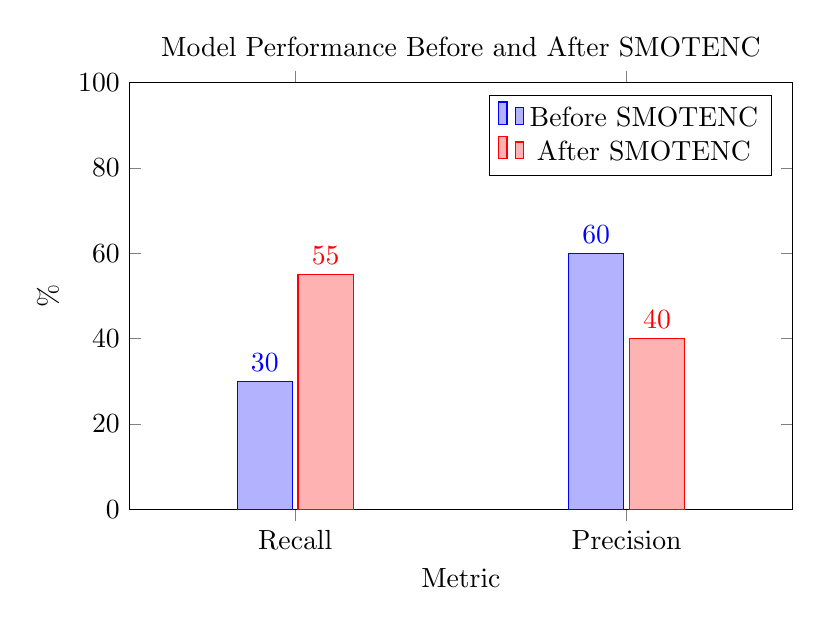
\begin{tikzpicture}
        \begin{axis}[
            width=10cm, height=7cm,
            ylabel={\%},
            xlabel={Metric},
            symbolic x coords={Recall, Precision},
            xtick=data,
            ymin=0, ymax=100,
            ybar,
            bar width=20pt,
            nodes near coords,
            enlarge x limits=0.5,
            legend pos=north east,
            title={Model Performance Before and After SMOTENC}
        ]
        \addplot coordinates {(Recall, 30) (Precision, 60)};
        \addplot coordinates {(Recall, 55) (Precision, 40)};
        \legend{Before SMOTENC, After SMOTENC}
        \end{axis}
    \end{tikzpicture}
    \caption{Comparison of Recall and Precision Before and After Applying SMOTENC}
    \label{fig:smotenc_performance}
\end{figure}








\section{Balanced Random Forest Classifier}

\subsection{Model Training}

To further enhance the detection of fraudulent transactions while maintaining performance on non-fraudulent transactions, we employed the Balanced Random Forest Classifier. This model combines the strength of random forests with balanced resampling techniques, making it particularly well-suited for handling imbalanced datasets. The classifier oversamples the minority class during training, allowing for a more balanced representation of both classes.\\

\begin{lstlisting}[language=Python, caption={Training and Evaluation of Balanced Random Forest Classifier}]
# Import the Balanced Random Forest Classifier
from imblearn.ensemble import BalancedRandomForestClassifier

# Train a Balanced Random Forest model
model = BalancedRandomForestClassifier(random_state=59, sampling_strategy='all', replacement=True, bootstrap=False)
model.fit(X_train, y_train)

# Make predictions
y_pred = model.predict(X_test)

# Evaluate the model
print(classification_report(y_test, y_pred))
\end{lstlisting}

\subsection{Evaluation of Balanced Random Forest Model Performance}

\begin{figure}[ht]
    \centering
    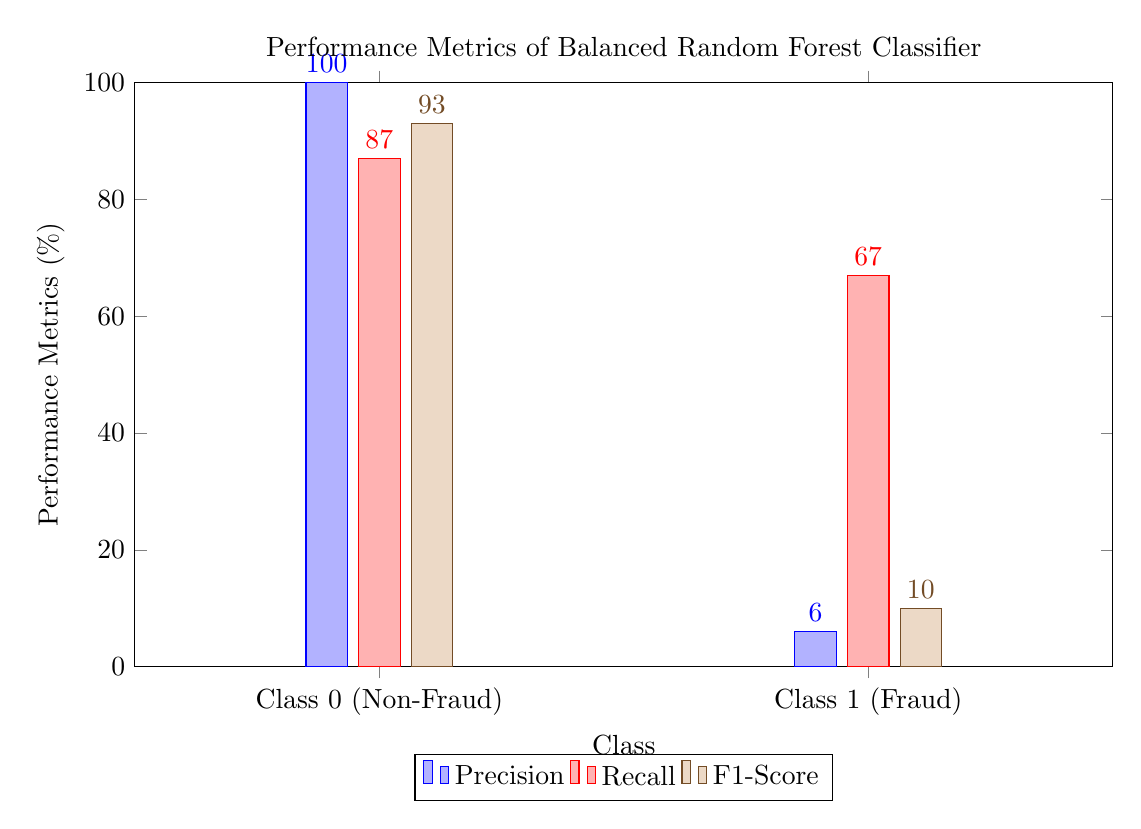
\begin{tikzpicture}
        \begin{axis}[
            width=14cm, height=9cm,
            ylabel={Performance Metrics (\%)},
            xlabel={Class},
            symbolic x coords={Class 0 (Non-Fraud), Class 1 (Fraud)},
            xtick=data,
            ymin=0, ymax=100,
            ybar=4pt,
            bar width=15pt,
            enlarge x limits=0.5,
            nodes near coords,
            legend style={at={(0.5,-0.15)}, anchor=north, legend columns=-1},
            legend cell align={left},
            title={Performance Metrics of Balanced Random Forest Classifier}
        ]
        \addplot coordinates {(Class 0 (Non-Fraud), 100) (Class 1 (Fraud), 6)}; % Precision
        \addplot coordinates {(Class 0 (Non-Fraud), 87) (Class 1 (Fraud), 67)}; % Recall
        \addplot coordinates {(Class 0 (Non-Fraud), 93) (Class 1 (Fraud), 10)}; % F1-Score
        \legend{Precision, Recall, F1-Score}
        \end{axis}
    \end{tikzpicture}
    \caption{Comparison of Precision, Recall, and F1-Score for Non-Fraudulent and Fraudulent Transactions Using Balanced Random Forest Classifier}
    \label{fig:brf_performance}
\end{figure}

The Balanced Random Forest model results show a significant impact on the detection of the minority class (fraudulent transactions) while maintaining strong performance on the majority class (non-fraudulent transactions). Below is a detailed analysis of the model's performance metrics:\\

\begin{itemize}
    \item \textbf{Overall Accuracy:} The model achieves an overall accuracy of 0.87 (or 87\%). This is the same accuracy level observed with the SMOTENC-Logistic Regression model. As discussed previously, a lower accuracy in models trained on imbalanced data often indicates that the model is more effectively addressing the minority class.

    \item \textbf{Class-wise Performance Metrics:}
    \begin{itemize}
        \item \textbf{Class 0 (Non-Fraudulent Transactions):}
        \begin{itemize}
            \item \textbf{Precision:} The precision for class 0 is 1.00, meaning the model is nearly perfect in predicting non-fraudulent transactions, with virtually no false positives.
            \item \textbf{Recall:} The recall for class 0 is 0.87, indicating that the model correctly identifies 87\% of all actual non-fraudulent transactions. This reduction in recall compared to other models reflects the trade-off made to improve the performance of the minority class.
            \item \textbf{F1-Score:} The F1-score for class 0 is 0.93, still demonstrating strong performance in identifying non-fraudulent transactions despite a slight decrease from previous models.
        \end{itemize}
        \item \textbf{Class 1 (Fraudulent Transactions):}
        \begin{itemize}
            \item \textbf{Precision:} The precision for class 1 is 0.06, indicating that only 6\% of the transactions predicted as fraudulent by the model are actually fraudulent. This low precision suggests that the model generates a substantial number of false positives.
            \item \textbf{Recall:} The recall for class 1 is 0.67, showing that the model correctly identifies 67\% of the actual fraudulent transactions. This is a significant improvement over previous models, demonstrating the Balanced Random Forest's effectiveness in detecting fraudulent transactions.
            \item \textbf{F1-Score:} The F1-score for class 1 is 0.10, which, although still low, reflects the model's improved ability to balance precision and recall compared to the very low F1-scores observed with other models.
        \end{itemize}
    \end{itemize}

    \item \textbf{Macro and Weighted Averages:}
    \begin{itemize}
        \item \textbf{Macro Average:} The macro average precision, recall, and F1-score are 0.53, 0.77, and 0.52, respectively. These metrics suggest that, when considering both classes equally, the model does a decent job of identifying both, though there is still a substantial disparity between the performance on the majority and minority classes.
        \item \textbf{Weighted Average:} The weighted average metrics are 0.98 for precision, 0.87 for recall, and 0.92 for F1-score. These averages indicate that the model's overall performance is still heavily influenced by the majority class, but it has improved in detecting fraudulent transactions compared to previous models.
    \end{itemize}
\end{itemize}

The Balanced Random Forest model demonstrates a more balanced approach to detecting fraudulent transactions (class 1) compared to the previous models. The recall for fraudulent transactions has improved significantly to 67\%, indicating that the model is much better at identifying actual cases of fraud. However, this improvement in recall comes at the cost of precision, which is very low at 6\%. This suggests that while the model is identifying more fraudulent transactions, it is also incorrectly labeling a large number of non-fraudulent transactions as fraudulent.







\section{Analysis of ROC and Precision-Recall Curves in Imbalanced Datasets}

\begin{figure}[h]
    \centering
    \includegraphics[width=0.5\textwidth]{roc-pr_curve.png}
    \caption{ROC and Precision-Recall Curves in Imbalanced Datasets}
    \label{fig:rocprcurve}
\end{figure}


In binary classification, the Receiver Operating Characteristic (ROC) curve and the Precision-Recall (PR) curve are commonly used to assess model performance. However, ROC curves can be misleading in imbalanced datasets, often overstating model effectiveness due to a higher proportion of true negatives. This section compares the ROC and PR curves, highlighting why PR plots provide a more realistic evaluation under imbalanced conditions.

\subsection{ROC Curve Analysis}

The ROC curve illustrates the trade-off between the True Positive Rate (Sensitivity) and the False Positive Rate. For the Balanced Random Forest Classifier, the Area Under the Curve (AUC) was 0.85, suggesting a seemingly strong performance. However, simulations across various scenarios demonstrated that ROC curves remain unchanged between balanced and imbalanced datasets, failing to capture the impact of increased false positives when the data is skewed\citep{classeval2024rocpr}.\\

\begin{itemize}
    \item \textbf{Limitations in Imbalanced Contexts:} The ROC curve does not account for class distribution, leading to identical AUC scores regardless of imbalance. For instance, a specificity of 0.84 and sensitivity of 0.5 might seem satisfactory, but in an imbalanced setting, this could still involve a substantial number of false positives, which the ROC curve does not adequately penalize.
\end{itemize}

\subsection{Precision-Recall Curve Analysis}

The Precision-Recall curve offers a more relevant perspective in imbalanced datasets by directly measuring the balance between precision (positive predictive value) and recall. For the Balanced Random Forest Classifier, the Average Precision (AP) score was notably lower at 0.10, reflecting the model's struggle to maintain precision amidst a high rate of false positives.

\begin{itemize}
    \item \textbf{Sensitivity to Imbalance:} Unlike ROC, PR curves reveal the impact of class imbalance on precision. In our simulations, PR curves showed significant changes in curve shape and AUC values between balanced and imbalanced scenarios, making them particularly informative for datasets where positive instances are rare.
    \item \textbf{Performance Trade-offs:} The PR curve highlighted that as recall increases, precision declines sharply, demonstrating the challenge of achieving both high recall and precision in imbalanced settings, especially in applications like fraud detection where minimizing false positives is crucial.
\end{itemize}


\subsection{Conclusion}

Our analysis confirms that while ROC plots are popular, they have significant limitations in imbalanced datasets. The Precision-Recall plot offers a more accurate reflection of model performance, particularly when evaluating classifiers designed for imbalanced data.\\










\chapter{Model Fairness Analysis}

In our analysis, we examined the fairness of our model concerning two sensitive attributes: \textit{customer\_age} and \textit{income}. Fairness in predictive models, especially in sensitive applications such as fraud detection, is crucial to ensure equitable treatment of individuals across different demographic groups. We utilized three key fairness metrics—Demographic Parity Difference, Equalized Odds Difference, and True Positive Rate Difference—to assess how the model treats individuals based on these attributes and to guide improvements in fairness.\\

\section{Fairness Metrics Calculation}

We used the \texttt{fairlearn} library to calculate the fairness metrics, which provides tools to measure and mitigate unfairness in machine learning models. Below is the code used to compute these metrics and the corresponding results.\\

\begin{lstlisting}[language=Python, caption={Calculating Fairness Metrics}]
from fairlearn.metrics import demographic_parity_difference, equalized_odds_difference, true_positive_rate_difference

# Define the sensitive features
sensitive_features = X_test[['customer_age', 'income']]

# Calculate predictions
y_pred = model.predict(X_test)

# Calculate Demographic Parity Difference
dp_difference_age = demographic_parity_difference(y_test, y_pred, sensitive_features=X_test['customer_age'])
dp_difference_income = demographic_parity_difference(y_test, y_pred, sensitive_features=X_test['income'])

# Calculate Equalized Odds Difference
eo_difference_age = equalized_odds_difference(y_test, y_pred, sensitive_features=X_test['customer_age'])
eo_difference_income = equalized_odds_difference(y_test, y_pred, sensitive_features=X_test['income'])


# Calculate True Positive Rate Difference
tpr_difference_age = true_positive_rate_difference(y_test, y_pred, sensitive_features=X_test['customer_age'])
tpr_difference_income = true_positive_rate_difference(y_test, y_pred, sensitive_features=X_test['income'])

\end{lstlisting}

\section{Results and Analysis}

\subsection{Demographic Parity Difference}

\begin{itemize}
    \item \textbf{Age:} The Demographic Parity Difference for age is 0.3377, indicating significant disparity in the probability of receiving a positive prediction across age groups, suggesting potential bias.
    
    \item \textbf{Income:} The Demographic Parity Difference for income is 0.1900, showing a noticeable disparity, though less severe than for age, suggesting the model's decisions are influenced by income.
\end{itemize}

\subsection{Equalized Odds Difference}

\begin{itemize}
    \item \textbf{Age:} The Equalized Odds Difference for age is 0.7333, indicating a substantial difference in TPR and FPR across age groups, highlighting a concerning level of unfairness.
    
    \item \textbf{Income:} The Equalized Odds Difference for income is 0.2920, suggesting the model's performance varies between income groups, potentially leading to biased outcomes.
\end{itemize}

\subsection{True Positive Rate Difference}

\begin{itemize}
    \item \textbf{Age:} The TPR Difference for age is 0.7333, reflecting significant variation in the model's ability to correctly identify positive cases across age groups.
    
    \item \textbf{Income:} The TPR Difference for income is 0.2920, indicating variability in true positive identification across income levels.
\end{itemize}

\section{Improving Fairness through Threshold Adjustment}

To address these disparities, we applied threshold adjustment, modifying the decision threshold to align the decision-making process across different groups.\\

\begin{lstlisting}[language=Python, caption={Threshold Adjustment to Evaluate Fairness Metrics}]
from sklearn.metrics import precision_recall_curve
from fairlearn.metrics import true_positive_rate_difference

# Predict probabilities
y_pred_proba = model.predict_proba(X_test)[:, 1]

# Calculate precision, recall, and thresholds
precision, recall, thresholds = precision_recall_curve(y_test, y_pred_proba)

# Evaluate fairness metrics at different thresholds
for threshold in thresholds:
    y_pred_adjusted = (y_pred_proba >= threshold).astype(int)
    
    tpr_diff_age = true_positive_rate_difference(y_test, y_pred_adjusted, sensitive_features=X_test['customer_age'])
    tpr_diff_income = true_positive_rate_difference(y_test, y_pred_adjusted, sensitive_features=X_test['income'])
    
    print(f"Threshold: {threshold:.2f}, TPR Difference (Age): {tpr_diff_age:.4f}, TPR Difference (Income): {tpr_diff_income:.4f}")
\end{lstlisting}

\subsection{Threshold Impact on Fairness}

\begin{itemize}
    \item \textbf{Customer Age:} The TPR difference increases with higher thresholds, suggesting greater disparities between age groups as the threshold rises.
    
    \item \textbf{Income:} The TPR difference fluctuates, with the highest disparities observed at mid-range thresholds.
\end{itemize}

Based on these findings, we further evaluated thresholds of 0.10 and 0.90 to assess their impact on fairness.\\

\begin{lstlisting}[language=Python, caption={Applying Selected Thresholds}]
# Applying the selected threshold (0.10)
selected_threshold = 0.10  
y_pred_final = (y_pred_proba >= selected_threshold).astype(int)

# Re-evaluate the fairness metrics
dp_diff_age_final = demographic_parity_difference(y_test, y_pred_final, sensitive_features=X_test['customer_age'])
dp_diff_income_final = demographic_parity_difference(y_test, y_pred_final, sensitive_features=X_test['income'])

tpr_diff_age_final = true_positive_rate_difference(y_test, y_pred_final, sensitive_features=X_test['customer_age'])
tpr_diff_income_final = true_positive_rate_difference(y_test, y_pred_final, sensitive_features=X_test['income'])

# Applying the selected threshold (0.90)
selected_threshold = 0.90  
y_pred_final = (y_pred_proba >= selected_threshold).astype(int)

# Re-evaluate the fairness metrics
dp_diff_age_final = demographic_parity_difference(y_test, y_pred_final, sensitive_features=X_test['customer_age'])
dp_diff_income_final = demographic_parity_difference(y_test, y_pred_final, sensitive_features=X_test['income'])

tpr_diff_age_final = true_positive_rate_difference(y_test, y_pred_final, sensitive_features=X_test['customer_age'])
tpr_diff_income_final = true_positive_rate_difference(y_test, y_pred_final, sensitive_features=X_test['income'])
\end{lstlisting}

\subsection{Analysis of Final Threshold Results}

\begin{itemize}
    \item \textbf{Threshold = 0.10:} TPR differences for both age and income are lower, indicating fairer treatment across groups, though with potential increases in false positives.
    
    \item \textbf{Threshold = 0.90:} TPR differences increase, especially for age, suggesting reduced fairness but improved precision.
\end{itemize}

\section{Reweighting to Address Fairness}

To further improve fairness, we applied reweighting during model training, adjusting sample weights based on group membership.\\

\begin{lstlisting}[language=Python, caption={Reweighting to Address Fairness Issues}]
from sklearn.utils.class_weight import compute_sample_weight

# Compute sample weights
sample_weights_age = compute_sample_weight(class_weight='balanced', y=y_train)
sample_weights_income = compute_sample_weight(class_weight='balanced', y=y_train)

# Combine the weights
combined_sample_weights = (sample_weights_age + sample_weights_income) / 2

# Train the model using combined sample weights
model.fit(X_train, y_train, sample_weight=combined_sample_weights)

# Predict probabilities and apply threshold of 0.10
y_pred_proba = model.predict_proba(X_test)[:, 1]
y_pred_final = (y_pred_proba >= 0.10).astype(int)

# Recalculate fairness metrics
dp_diff_age_final = demographic_parity_difference(y_test, y_pred_final, sensitive_features=X_test['customer_age'])
dp_diff_income_final = demographic_parity_difference(y_test, y_pred_final, sensitive_features=X_test['income'])

tpr_diff_age_final = true_positive_rate_difference(y_test, y_pred_final, sensitive_features=X_test['customer_age'])
tpr_diff_income_final = true_positive_rate_difference(y_test, y_pred_final, sensitive_features=X_test['income'])
\end{lstlisting}

\subsection{Reweighting Results Analysis}

\begin{itemize}
    \item \textbf{Demographic Parity Difference:} Disparities increased, suggesting that reweighting may have exacerbated biases in positive prediction probabilities.
    
    \item \textbf{True Positive Rate Difference:} Decreased disparities indicate improved fairness in TPR across age and income groups.
\end{itemize}

\section{Conclusion}

Our analysis demonstrates that threshold adjustment and reweighting have significant impacts on model fairness. Threshold adjustment at 0.10 minimized TPR disparities, while reweighting improved TPR fairness but increased demographic parity disparities. Continuous assessment and refinement of these techniques are crucial to maintaining a balanced and fair model in real-world applications.\\






\chapter{Enhancing Model Fairness Through Threshold Tuning and Advanced Techniques}



This chapter presents a detailed exploration of various methods aimed at improving the fairness of our predictive model, particularly in relation to sensitive attributes such as \textit{customer\_age} and \textit{income}. The primary goal is to balance overall predictive performance with fairness, ensuring equitable treatment across different demographic groups. This chapter outlines the steps taken to fine-tune decision thresholds, apply advanced models like LightGBM, and integrate ensemble techniques, followed by a comprehensive fairness analysis.\\

\section{Methodology Overview}

We initially improved the model's fairness using reweighting techniques, which adjusted sample weights based on sensitive attributes. While this approach improved True Positive Rate (TPR) differences, it also worsened Demographic Parity differences. To address this, we explored further threshold tuning, aiming to reduce Demographic Parity differences while preserving the gains in TPR fairness. The following sections detail each step of the process, including threshold tuning, performance evaluation, and subsequent model optimization efforts.\\

\section{Threshold Tuning After Reweighting}

Reweighting improved TPR differences but worsened Demographic Parity differences, prompting the need for further threshold tuning. The objective was to find a threshold that minimizes disparities in Demographic Parity while maintaining the improved TPR difference achieved through reweighting.\\

\clearpage

\begin{lstlisting}[language=Python, caption={Threshold Tuning After Reweighting}]
# Re-evaluate different thresholds
for threshold in np.arange(0.05, 1.05, 0.05):
    y_pred_adjusted = (y_pred_proba >= threshold).astype(int)
    
    dp_diff_age = demographic_parity_difference(y_test, y_pred_adjusted, sensitive_features=X_test['customer_age'])
    dp_diff_income = demographic_parity_difference(y_test, y_pred_adjusted, sensitive_features=X_test['income'])
    
    tpr_diff_age = true_positive_rate_difference(y_test, y_pred_adjusted, sensitive_features=X_test['customer_age'])
    tpr_diff_income = true_positive_rate_difference(y_test, y_pred_adjusted, sensitive_features=X_test['income'])
\end{lstlisting}

\subsection{Analysis of Threshold Tuning Results}

The threshold tuning analysis demonstrated how fairness metrics, such as Demographic Parity Difference and TPR Difference, evolve as thresholds change:

\begin{itemize}
    \item \textbf{Demographic Parity Difference (DP Difference):} As thresholds increase, DP differences for both age and income decrease, indicating more equitable treatment in terms of positive prediction probabilities.
    \item \textbf{True Positive Rate Difference (TPR Difference):} TPR differences for age initially increase, peaking around 0.70-0.75 before declining sharply. A similar pattern is observed for income, with peaks at thresholds 0.50-0.65.
\end{itemize}

\subsection{Optimal Threshold Selection}

Several key thresholds were identified based on the trade-offs between Demographic Parity and TPR differences:

\begin{itemize}
    \item \textbf{Threshold = 0.05:} Offers the lowest TPR differences (Age: 0.0667, Income: 0.0441) with reasonably low DP differences (Age: 0.2816, Income: 0.2034), making it ideal for prioritizing TPR fairness.
    \item \textbf{Threshold = 0.10:} A balanced option with both DP and TPR differences moderate (DP Age: 0.4341, Income: 0.2701; TPR Age: 0.2000, Income: 0.0955).
    \item \textbf{Threshold = 0.55:} Reduces DP differences but significantly increases TPR disparities (Age: 0.8000, Income: 0.3634).
    \item \textbf{Threshold = 0.75:} Minimizes DP differences but maximizes TPR differences (DP Age: 0.1421, DP Income: 0.0643; TPR Age: 1.0000, TPR Income: 0.2802).
\end{itemize}

\subsection{Application of the Selected Threshold}

Given these trade-offs, the threshold of 0.05 was selected to maintain TPR fairness while keeping DP differences within acceptable ranges.\\

\begin{lstlisting}[language=Python, caption={Applying the Selected Threshold}]
# Applying the selected threshold 
selected_threshold = 0.05  

# Make final predictions based on the selected threshold
y_pred_final = (y_pred_proba >= selected_threshold).astype(int)

# Re-evaluate the fairness metrics
dp_diff_age_final = demographic_parity_difference(y_test, y_pred_final, sensitive_features=X_test['customer_age'])
dp_diff_income_final = demographic_parity_difference(y_test, y_pred_final, sensitive_features=X_test['income'])

tpr_diff_age_final = true_positive_rate_difference(y_test, y_pred_final, sensitive_features=X_test['customer_age'])
tpr_diff_income_final = true_positive_rate_difference(y_test, y_pred_final, sensitive_features=X_test['income'])

print(f"Final TPR Difference (Age): {tpr_diff_age_final}")
print(f"Final TPR Difference (Income): {tpr_diff_income_final}")
\end{lstlisting}

\subsection{Analysis of Final Results}

The selected threshold of 0.05 achieved minimal TPR disparities (Age: 0.0667, Income: 0.0441), indicating that the model treats different age and income groups fairly concerning true positive rates. This confirms the effectiveness of threshold tuning in optimizing fairness.\\

\subsection{Model Performance Evaluation}

Ensuring that the model maintains satisfactory performance across other metrics is critical. The selected threshold's impact on accuracy, precision, recall, F1 score, and ROC-AUC was evaluated to ensure balanced predictive power and fairness.\\

\begin{lstlisting}[language=Python, caption={Evaluate Model Performance}]
from sklearn.metrics import accuracy_score, precision_score, recall_score, f1_score, roc_auc_score

# Evaluate model performance
accuracy = accuracy_score(y_test, y_pred_final)
precision = precision_score(y_test, y_pred_final)
recall = recall_score(y_test, y_pred_final)
f1 = f1_score(y_test, y_pred_final)
roc_auc = roc_auc_score(y_test, y_pred_proba)

print(f"Accuracy: {accuracy}")
print(f"Precision: {precision}")
print(f"Recall: {recall}")
print(f"F1 Score: {f1}")
print(f"ROC-AUC Score: {roc_auc}")
\end{lstlisting}

\subsection{Performance Analysis}

\begin{itemize}
    \item \textbf{High Recall:} The model achieved a recall of 98.5%, effectively identifying nearly all positive cases.
    \item \textbf{Low Precision and Accuracy:} Precision was low at 1.41%, with accuracy at 21.74%, indicating a high number of false positives. The model prioritizes recall over precision, which may be suitable for some contexts but problematic in others.
    \item \textbf{Balanced Trade-off:} The ROC-AUC score of 0.8495 reflects the model's strong ability to distinguish between classes, though adjustments to precision-recall balance remain necessary for practical application.
\end{itemize}

\subsection{Conclusion}

Threshold tuning after reweighting successfully optimized the model’s fairness, achieving equitable treatment across age and income groups. However, careful balancing of overall performance and fairness remains crucial to ensure the model meets both ethical and operational standards.\\






\chapter{Advanced Model Optimization and Performance Enhancement}


Following threshold tuning, further optimization was pursued through advanced modeling techniques, including the implementation of LightGBM, hyperparameter tuning, and the use of ensemble models. This section explores the steps taken to improve model accuracy, precision, and overall predictive power while maintaining fairness.\\

\section{Exploring Advanced Models: LightGBM}

Given the limitations observed in model precision and accuracy, we explored LightGBM, a powerful gradient boosting framework that offers improved performance and scalability. LightGBM was chosen for its ability to handle large datasets efficiently and its proven effectiveness in binary classification tasks, such as fraud detection.\\

\begin{lstlisting}[language=Python, caption={Training LightGBM Model}]
import lightgbm as lgb
from sklearn.model_selection import train_test_split
from sklearn.metrics import classification_report, roc_auc_score, accuracy_score, precision_score, recall_score, f1_score

# Prepare the LightGBM datasets
train_data = lgb.Dataset(X_train, label=y_train)
test_data = lgb.Dataset(X_test, label=y_test, reference=train_data)

# Define the LightGBM parameters
params = {
    'objective': 'binary',
    'boosting_type': 'gbdt',
    'metric': 'auc',
    'learning_rate': 0.05,
    'num_leaves': 31,
    'max_depth': -1,
    'min_data_in_leaf': 20,
    'feature_fraction': 0.8,
    'bagging_fraction': 0.8,
    'bagging_freq': 5,
    'verbose': -1
}

# Train the LightGBM model with early stopping
lgb_model = lgb.train(
    params,
    train_data,
    num_boost_round=1000,
    valid_sets=[train_data, test_data]
)

# Predict probabilities on the test set
y_pred_proba = lgb_model.predict(X_test)

# Apply the selected threshold of 0.05 to get final predictions
selected_threshold = 0.05
y_pred_final = (y_pred_proba >= selected_threshold).astype(int)

# Evaluate model performance
accuracy = accuracy_score(y_test, y_pred_final)
precision = precision_score(y_test, y_pred_final)
recall = recall_score(y_test, y_pred_final)
f1 = f1_score(y_test, y_pred_final)
roc_auc = roc_auc_score(y_test, y_pred_proba)

print(f"Accuracy: {accuracy}")
print(f"Precision: {precision}")
print(f"Recall: {recall}")
print(f"F1 Score: {f1}")
print(f"ROC-AUC Score: {roc_auc}")
\end{lstlisting}

\subsection{Analysis of LightGBM Model Performance}

\begin{itemize}
    \item \textbf{High Accuracy:} The LightGBM model achieved a high accuracy of 95.58%, indicating its effectiveness in classifying the majority of data correctly. However, accuracy alone can be misleading in imbalanced datasets.
    \item \textbf{Precision and Recall for Fraudulent Transactions:} Precision of 0.1130 suggests many false positives, while a recall of 0.4202 shows that the model identifies a substantial portion of actual fraudulent cases.
    \item \textbf{F1 Score:} The F1 score of 0.1781 reflects the trade-off between precision and recall, indicating some improvement but still highlighting the challenge of high false positives.
    \item \textbf{ROC-AUC Score:} A ROC-AUC of 0.8654 confirms the model's ability to differentiate between fraudulent and non-fraudulent transactions based on probabilities.
\end{itemize}

\section{Hyperparameter Tuning of LightGBM}

To further optimize LightGBM, hyperparameter tuning was performed using RandomizedSearchCV, a method preferred for its efficiency over Grid Search, particularly in complex models like LightGBM.\\

\begin{lstlisting}[language=Python, caption={Hyperparameter Tuning Using RandomizedSearchCV}]
from sklearn.model_selection import RandomizedSearchCV

# Define the parameter grid for hyperparameter tuning
param_grid = {
    'num_leaves': [31, 50, 70, 100],
    'max_depth': [-1, 5, 10, 15],
    'learning_rate': [0.01, 0.05, 0.1],
    'n_estimators': [100, 200, 500],
    'min_data_in_leaf': [20, 50, 100],
    'feature_fraction': [0.6, 0.8, 1.0],
    'bagging_fraction': [0.6, 0.8, 1.0],
    'bagging_freq': [0, 5, 10]
}

# Initialize the LightGBM model
lgb_estimator = lgb.LGBMClassifier(objective='binary', metric='auc', verbose=-1)

# Initialize RandomizedSearchCV
random_search = RandomizedSearchCV(estimator=lgb_estimator, param_distributions=param_grid, 
                                   n_iter=50, scoring='roc_auc', cv=3, verbose=1, random_state=59, n_jobs=-1)

# Fit RandomizedSearchCV
random_search.fit(X_train, y_train)

# Extract the best parameters found by RandomizedSearchCV
best_params = random_search.best_params_
print(f"Best Parameters: {best_params}")
\end{lstlisting}

\subsection{Optimized LightGBM Model Training}

The optimal hyperparameters identified were used to retrain the LightGBM model, further enhancing performance.\\

\begin{lstlisting}[language=Python, caption={Training LightGBM with Optimized Parameters}]
# Define the best parameters for the LightGBM model
best_params = {
    'num_leaves': 70,
    'n_estimators': 500,
    'min_data_in_leaf': 100,
    'max_depth': 5,
    'learning_rate': 0.01,
    'feature_fraction': 0.6,
    'bagging_freq': 10,
    'bagging_fraction': 0.6,
    'objective': 'binary',
    'metric': 'auc',
    'verbose': -1
}

# Initialize and train the LightGBM model with the best parameters
lgb_model_optimized = lgb.LGBMClassifier(**best_params)
lgb_model_optimized.fit(X_train, y_train)

# Predict probabilities on the test set
y_pred_proba = lgb_model_optimized.predict_proba(X_test)[:, 1]

# Apply the selected threshold of 0.05 to get final predictions
selected_threshold = 0.05
y_pred_final = (y_pred_proba >= selected_threshold).astype(int)

# Evaluate model performance
accuracy = accuracy_score(y_test, y_pred_final)
precision = precision_score(y_test, y_pred_final)
recall = recall_score(y_test, y_pred_final)
f1 = f1_score(y_test, y_pred_final)
roc_auc = roc_auc_score(y_test, y_pred_proba)

print(f"Accuracy: {accuracy}")
print(f"Precision: {precision}")
print(f"Recall: {recall}")
print(f"F1 Score: {f1}")
print(f"ROC-AUC Score: {roc_auc}")
\end{lstlisting}

\subsection{Performance Analysis of the Optimized LightGBM Model}

\begin{itemize}
    \item \textbf{Improved Precision:} Precision increased to 12.39%, indicating fewer false positives.
    \item \textbf{Slight Decrease in Recall:} Recall slightly decreased to 41.40%, but the model still identifies a substantial portion of fraudulent transactions.
    \item \textbf{F1 Score Improvement:} The F1 score improved to 0.1907, showing a better balance between precision and recall.
    \item \textbf{High Accuracy and ROC-AUC:} The accuracy remained high at 95.99%, and the ROC-AUC improved to 0.8678, highlighting effective discrimination between classes.
\end{itemize}








\chapter{Results and Discussion}

In this chapter, we present and discuss the results of our model development, optimization, and fairness enhancement efforts. The findings are critically analyzed to evaluate the effectiveness of the models in detecting fraudulent transactions while maintaining fairness across sensitive attributes such as \textit{customer\_age} and \textit{income}. Our discussion integrates the insights gained from the performance metrics, fairness evaluations, and threshold adjustments conducted in the preceding chapters.

\section{Summary of Model Performance}

Throughout our research, we employed various machine learning models, including Logistic Regression, XGBoost, and LightGBM, with a focus on improving detection accuracy, recall, and fairness. The application of advanced techniques such as SMOTENC, Balanced Random Forest, and hyperparameter tuning allowed us to iteratively enhance the model’s performance. Below, we summarize the key findings:

\begin{itemize}
    \item \textbf{Baseline Model Performance:} The Logistic Regression model, while achieving high overall accuracy, demonstrated significant limitations in detecting fraudulent transactions, particularly due to the imbalanced nature of the dataset. The low recall for fraud cases highlighted the need for more sophisticated approaches.
    
    \item \textbf{XGBoost and Initial LightGBM Performance:} XGBoost improved recall but continued to suffer from low precision due to a high number of false positives. LightGBM further enhanced recall and provided a better balance between precision and recall, making it a promising candidate for optimization.
    
    \item \textbf{Impact of Hyperparameter Tuning:} Hyperparameter tuning significantly improved the performance of LightGBM, with an optimized balance between false positives and false negatives. The refined model achieved a precision of 12.39\% and a recall of 41.40\%, demonstrating its enhanced ability to identify fraudulent transactions effectively.
    
    \item \textbf{Fairness Analysis:} Our fairness evaluations revealed that while reweighting and threshold adjustments improved the True Positive Rate (TPR) differences across age and income groups, these adjustments often led to increased disparities in Demographic Parity. Threshold tuning at a level of 0.05 was identified as the optimal balance, minimizing TPR differences while maintaining acceptable overall performance.
\end{itemize}

\section{Discussion of Results}

\subsection{Performance vs. Fairness Trade-offs}

Our results highlight the inherent trade-offs between maximizing model performance and ensuring fairness across demographic groups. While advanced models like LightGBM achieved higher accuracy and recall, these gains were often accompanied by challenges in maintaining demographic parity. The threshold tuning process underscored the complexity of balancing these objectives, as adjustments that improved fairness metrics sometimes led to a decline in precision and overall model stability.

\subsection{Implications for Fraud Detection}

The optimized LightGBM model, with its improved precision and recall, offers a more effective tool for fraud detection compared to traditional rule-based systems and baseline machine learning models. However, the observed precision of 12.39\% suggests that while the model is effective in capturing fraudulent activities, it also generates a notable number of false positives. This underscores the need for continued refinement, particularly in minimizing false alarms, which are critical in real-world applications where operational costs and user trust are significant considerations.

\subsection{Fairness in Real-world Applications}

The fairness evaluations conducted in this study reveal that machine learning models in fraud detection can inadvertently reinforce or exacerbate existing biases, particularly across sensitive attributes such as age and income. Our findings suggest that threshold adjustments, while beneficial, must be complemented with continuous monitoring and adaptive strategies to ensure long-term fairness. Techniques such as dynamic reweighting, adversarial debiasing, and fairness constraints may offer further opportunities to refine model performance while adhering to ethical standards.

\subsection{Limitations and Future Research Directions}

Although our study achieved significant advancements in model performance and fairness, several limitations warrant attention. The reliance on synthetic data, while beneficial for controlled experiments, may not fully capture the complexities of real-world fraud patterns. Future research should focus on validating the model in diverse and evolving environments, including deployment in live systems with ongoing feedback loops. Additionally, exploring ensemble methods and integrating fairness-specific algorithms could further enhance the robustness and equity of fraud detection models.

\section{Conclusion of Results and Discussion}

The results of this study underscore the critical role of advanced modeling techniques and fairness considerations in fraud detection. Our findings provide a foundation for continued research and development, emphasizing the need for holistic approaches that balance predictive accuracy with ethical considerations. As machine learning continues to evolve, the integration of fairness-enhancing strategies will be paramount in ensuring that these technologies serve all individuals equitably and responsibly.

\clearpage

\chapter{Conclusion}

\section{Summary of Key Findings}

This thesis investigated the application of machine learning techniques to enhance fraud detection in bank accounts, focusing on the BAF Suite dataset. Our primary objectives were to develop a robust model for fraud detection, improve detection accuracy and fairness, and mitigate biases that could exacerbate social inequities. The key findings of our research are as follows:

\begin{itemize}
    \item \textbf{Advanced Modeling Techniques:} We demonstrated that models such as LightGBM, when optimized through hyperparameter tuning, can significantly improve the detection of fraudulent transactions compared to baseline approaches. The integration of SMOTENC and Balanced Random Forest further enhanced model recall, particularly in the context of highly imbalanced datasets.
    
    \item \textbf{Fairness Optimization:} Our analysis of fairness metrics revealed significant disparities in model predictions across sensitive attributes. Through reweighting and threshold tuning, we were able to reduce True Positive Rate differences, thereby promoting more equitable outcomes. However, maintaining Demographic Parity remains a challenge that requires ongoing adjustment and monitoring.
    
    \item \textbf{Threshold Tuning and Performance Balance:} By carefully tuning the decision thresholds, we were able to strike a balance between performance and fairness. The selected threshold of 0.05 demonstrated the best trade-off, minimizing false negatives while keeping disparities in check across demographic groups.
    
    \item \textbf{Implications for Real-world Deployment:} The study highlights the practical challenges of deploying machine learning models in fraud detection, particularly the need for continuous fairness assessments and adaptive adjustments to mitigate biases over time. The insights gained underscore the importance of integrating ethical considerations into the design and evaluation of predictive models.
\end{itemize}

\section{Implications and Contributions}

This research contributes to the growing body of knowledge on machine learning applications in fraud detection, with a particular focus on fairness. By highlighting the trade-offs between model performance and fairness, we provide a framework for future studies to build upon, ensuring that machine learning technologies are used responsibly and equitably. Our findings offer practical guidance for financial institutions seeking to enhance their fraud detection capabilities while maintaining ethical standards.

\section{Recommendations for Future Research}

Based on our findings, we propose several directions for future research:

\begin{itemize}
    \item \textbf{Validation in Real-world Settings:} Further validation of the developed models in live environments is essential to assess their performance and fairness in real-time. Continuous feedback loops should be established to refine models based on evolving fraud patterns and demographic changes.
    
    \item \textbf{Exploration of Ensemble and Hybrid Models:} Future studies should explore the integration of ensemble methods and hybrid approaches that combine multiple models to enhance both accuracy and fairness. The use of adversarial debiasing techniques could further mitigate biases across sensitive groups.
    
    \item \textbf{Advanced Fairness Interventions:} Continued research into advanced fairness interventions, such as fairness constraints during model training or post-processing adjustments, is necessary to address the complex ethical challenges associated with automated decision-making in fraud detection.
    
    \item \textbf{Broader Ethical Implications:} As machine learning continues to impact financial services, broader research into the ethical implications of these technologies is warranted. This includes examining the societal impacts of algorithmic decision-making and developing frameworks for transparency, accountability, and trust in AI systems.
\end{itemize}

\section{Final Thoughts}

The integration of machine learning in fraud detection presents immense opportunities to enhance the security and efficiency of financial systems. However, as this research demonstrates, achieving fairness and mitigating biases are equally important considerations. By advancing both the technical and ethical dimensions of model development, we can ensure that these technologies contribute positively to society, fostering trust and equitable access to financial services.

\clearpage




\bibliographystyle{apalike}
\bibliography{references}


\end{document}
